%%
%% Beuth Hochschule für Technik --  Abschlussarbeit
%%
%% Hauptdokument
%%
%% 23.01.09 Tschirley V.01
%% 24.08.14 Bergen V.03
%%
%%%%%%%%%%%%%%%%%%%%%%%%%%%%%%%%%%%%%%%%%%%%%%%%%%%%%%%%%%%%%%%%%%%%%
\documentclass[11pt, a4paper]{book}

%% Übersetzen als Entwurf
\usepackage[entwurf]{latexTemplate/bhtThesis}
%% Übersetzen für die Abgabe
%\usepackage[abgabe]{latexTemplate/bhtThesis}
\typeout{BHT-Abschlussarbeit V3 28.04.14 E.Bergen}
\usepackage{blindtext}   %für Blindtext, warum auch immer; ohne geht maketitle nicht: EB, 01.05.2014
\usepackage{listings}
\lstset{ 
  literate={ö}{{\"o}}1
           {ä}{{\"a}}1
           {ü}{{\"u}}1
           {Ö}{{\"O}}1
           {Ä}{{\"A}}1
           {Ü}{{\"U}}1
           {ß}{{\ss}}2
}

% Symbole
\usepackage{trsym} % http://ftp.gwdg.de/pub/ctan/fonts/trsym/trsym.pdf
\usepackage{bytefield} %http://ftp.uni-erlangen.de/mirrors/CTAN/macros/latex/contrib/bytefield/bf-example.pdf
\usepackage{bibgerm}
\usepackage{MnSymbol}
\usepackage{lmodern}
\usepackage{multibib}
%\usepackage[acronyms]{glossaries}
\usepackage[acronym,style=long,toc=true,numberedsection=autolabel]{glossaries} 
%\robustify{\gls}

\usepackage{booktabs}
\makeglossaries


\newcites{lit}{Literaturverzeichnis}
\newcites{int}{Internetquellen}

\usepackage{listings,xcolor}

\definecolor{listingBackground}{rgb}{0.97,0.97,0.97}
\definecolor{stringColor}{rgb}{0.37,0.37,0.37}
\lstset{
	basicstyle=\footnotesize\ttfamily,
	%numbers=left,
	numberstyle=\tiny,
	%stepnumber=2,
	numbersep=5pt,
	tabsize=2,
	extendedchars=true,
	breaklines=true,
	keywordstyle=\color{red},
	frame=b,
	stringstyle=\color{stringColor}\ttfamily,
	showspaces=false,
	showtabs=false,
	xleftmargin=17pt,
	framexleftmargin=17pt,
	framexrightmargin=5pt,
	framexbottommargin=4pt,
	backgroundcolor=\color{listingBackground},
	showstringspaces=false
}

\usepackage{caption}
\DeclareCaptionFont{white}{\color{black}}
\DeclareCaptionFormat{listing}{\colorbox[rgb]{0.87, 0.87, 0.87}{\parbox{\textwidth}{\hspace{15pt}#1#2#3}}}
\captionsetup[lstlisting]{format=listing,labelfont=white,textfont=white,singlelinecheck=false,margin=0pt,font={bf,footnotesize}}

\usepackage[babel,german=quotes]{csquotes}

\DeclareQuoteStyle{fquotes}
  {\em}{}{\em}{}

\newcommand*{\myfquote}[1]{%
  \begingroup%
    \setquotestyle{fquotes}%
    \enquote{#1}%
  \endgroup%
}

\newif\ifmyblockquote
\newcommand*{\myblockquote}{%
\myblockquotetrue\blockquote}

\DeclareQuoteStyle[italics]{german}
[\itshape]
[\itshape]
{\quotedblbase}
{\textquotedblleft}
[0.025em]
{\quotesinglbase}
{\fixligatures\textquoteleft}
\DeclareQuoteAlias[italics]{german}{german}


\renewcommand\mkblockquote[4]{\enquote{#1#2#3}#4}

%%
%% Pfad zu den Bildern
%%
\graphicspath{
  {pictures/},
  %{einleitung/pictures},
  %{kapitel1/pictures/},
  %{kapitel2/pictures/}
}

%%
%% Einbinden persönlicher macros 
%%
%
% Persönliche Macros
%
%

% Macros für Formeln
\newcommand{\jw}{j\omega}

% Begriffe

\newcommand{\OPV}{Operations\-ver\-stär\-ker}

\newcounter{itemlist}[chapter]
\renewcommand*{\theitemlist}{\thechapter.\arabic{itemlist}}

\newenvironment{itemlist}[2]{%
  \refstepcounter{itemlist}%  
  \hspace*{1em} \\ {Liste~\theitemlist ~-~#1:\ } \label{#2}	
  \begin{itemize}
}{%
  \end{itemize}
}

%% Message
\typeout{-----------------------------------------------------------}
\typeout{----> thesis.tex ---- Zentrales Dokument-------------------}
\typeout{-----------------------------------------------------------}

\version{MILESTONE 17 (MS17)}
\abgabedatum{{27}. {Oktober} {2014}}
%%
%% Titel, Autor und Betreuer
%%
\fachbereich{VI -- Informatik und Medien --} 
\studiengang{Medieninformatik-Online (Master)}
\autor{Eduard Bergen}
\matrnr{769248}
\titel{Vergleich von Streamingframeworks: \\ STORM, KAFKA, FLUME, S4}
\untertitel{}
\betreuerFeld{
  \begin{tabular}{llr}
    
    \textbf{1. Betreuer} & Herr~Prof.~Dr.~Edlich & Beuth Hochschule für Technik\\
    \textbf{Gutachter} & Herr~Prof.~Knabe & Beuth Hochschule für Technik
  \end{tabular}
}

%%\renewcommand{\baselinestretch}{1.05} 
\renewcommand{\arraystretch}{1.3}
\pagenumbering{Alph}
\begin{document}
\pagestyle{fancy}
\newacronym{glo:mpeg}{MPEG}{Motion Pictures Expert Group}
\newacronym{glo:tcp}{TCP}{Transmission Control Protocol}
\newacronym{glo:esp}{ESP}{Event Stream Processing}
\newacronym{glo:spe}{SPE}{Stream Processing Engine}
\newacronym[plural=RPCs,firstplural=Remote Procedure Calls (RPCs)]{glo:rpc}{RPC}{Remote Procedure Call}
\newacronym{glo:qos}{QoS}{Quality of Service}
\newacronym[plural=CPs, firstplural=Connection Points (CPs)]{glo:cp}{CP}{Connection Point}
\newacronym{glo:vecme}{VM}{Vector of Metrics}
\newacronym{glo:cap}{CAP}{Consistancy, Availability, Partition Tolerance}
\newacronym{glo:base}{BASE}{Basically Available, Soft State, Eventually Consistant}
\newacronym{glo:osi}{OSI}{Open Systems Interconnection Model}
\newacronym{glo:fk}{fk}{foreign key}
\newacronym{glo:pk}{pk}{primary key}
\newacronym{glo:k}{k}{key}
\newacronym{glo:v}{v}{value}
\newacronym{glo:orm}{ORM}{Object-relational mapping}
\newacronym{glo:xml}{XML}{Extensible Markup Language}
\newacronym{glo:coo}{C++}{C objektorientierte Programmiersprache}
\newacronym{glo:nmstl}{NMSTL}{Networking, Messaging, Servers, and Threading Library}
\newacronym{glo:antlr}{ANTLR}{ANother Tool for Language Recognition}
\newacronym{glo:cpu}{CPU}{Central Processing Unit}
\newacronym{glo:iso}{ISO}{International Organization for Standardization}
\newacronym{glo:asf}{ASF}{Apache Software Foundation}

\cleardoublepage

%%
%% Beuth Hochschule für Technik --  Abschlussarbeit
%%
%% Titelseiten und Erklärungen 
%%
%%%%%%%%%%%%%%%%%%%%%%%%%%%%%%%%%%%%%%%%%%%%%%%%%%%%%%%%%%%%%%%%%%%%%

\maketitle
\clearpage
\thispagestyle{empty}
% Rueckseite (leer)
%% 
~
\newpage

%%
%% Abstract
%%
%%%%%%%%%%%%%%%%%%%%%%%%%%%%%%%%%%%%%%%%%%%%%%%%%%%%%%%%%%%%%%%%%%%%%


\section*{Kurzfassung}
Mit der enormen Zunahme von Information in unterschiedlichen Quellen wie Sensoren (RFID) oder 
Nachrichtenquellen (RFD newsfeeds) wird es schwieriger Informationen beständig abzufragen. Um die
Frage zu klären, welcher Rechner am häufigsten in einem Netzwerk frequentiert wird, werden unterstützende 
Systeme notwendig. An dieser Stelle helfen Methoden aus dem Bereich des Complex Event Processing (CEP).
Im Spezialbereich Stream Processing von CEP wurden Streaming Frameworks entwickelt, 
um die Arbeit in der Datenflussverarbeitung zu unterstützen und damit komplexe Abfragen auf einer höheren
Schicht zu vereinfachen. In dieser Master Thesis geht es um einen Vergleich zwischen den Streaming Frameworks:
Apache Storm, Apache Kafka, Apache Flume und Apache S4. In der Thesis werden Prototypen entwickelt, um
Messwerte zu erfassen und zu vergleichen.



%% eof

%%
%% Abstract
%%
%%%%%%%%%%%%%%%%%%%%%%%%%%%%%%%%%%%%%%%%%%%%%%%%%%%%%%%%%%%%%%%%%%%%%


\section*{Abstract}
With the tremendous growth of information in various sources such as sensors (RFID) or news sources (RFD newsfeeds)
it is more difficult to query information continously. To clarify the question, which machine is most commonly frequented in a network, supporting systems are beeing necessary. At this point methods in the field of Complex Event Processing (CEP) help to solve this issue. In the special area of stream processing of CEP, streaming frameworks were developed to support and simplify the work of complex queries in a higher abstraction level. This master thesis involves a comaprison between the streaming frameworks: Apache Storm, Apache Kafka, Apache Flume and Apache S4. In the thesis prototypes are developed to capture and to compare measured values.

%% eof

%\clearpage

%\ifthenelse{\boolean{@entwurfset}}
%    {

%    }
%    {
%      ~
%      \newpage
%      \vfill
%      \section*{Aufgabenblatt -- durch Original austauschen !!!}
%      \vfill
%      \clearpage
%      ~
%      \newpage
%    }
%\vspace{10ex}
%\section*{Erklärung}
%Ich  versichere, dass  ich diese  Abschlussarbeit ohne  fremde  Hilfe selbstständig
%verfasst und  nur die  angegebenen Quellen und  Hilfsmittel benutzt  habe. Wörtlich
%oder dem  Sinn nach  aus anderen  Werken entnommene Stellen  sind unter  Angabe der
%Quellen kenntlich gemacht.
%\vspace{10ex}\\

%\hrule
%{\small{Datum}}\hfill{\small{Unterschrift}}


\pagenumbering{roman}
\tableofcontents
%\listoffigures
\frontmatter



\mainmatter

\pagenumbering{arabic}
%%%%%%%%%%%%%%%%%%%%%%%%%%%%%%%%%%%%%%%%%%%%%%%%%%%%%%%%%%%%%%%
%% Die Kapitel der Arbeit

\chapter{Einführung}

\begin{quote}
Social media streams, such as Twitter, have shown themselves to be useful sources of real-time information about what is happening in the world. Automatic detection and tracking of events identified in these streams have a variety of real-world applications, e.g. identifying and automatically reporting road accidents for emergency services.
\citelit{mccreadie2013scalable}
\end{quote}

Im Marktplatz Internet steigt das Angebot zu unterschiedlichen Informationen rapide an. Gerade in Deutschland wächst das Datenaufkommen anhand einer Studie der IDC \citelit[S. 2-3]{res:idcDuGer} exponentiell. Dabei nimmt ebenfalls das Interesse an wiederkehrenden Aussagen über die Anzahl bestimmter Produkte, die Beziehungen zu Personen und die persönlichen Stimmungen zueinander zu. Die Infografik \citeint{res:DataNeverSleeps20} von Josh James, Firma Domo zeigt wieviel und welche Art von Daten in einer Minute an unterschiedlichen Stellen im Internet erzeugt werden. 

Um die Sicherheit bei Verlust einer Kreditkarte zu erhöhen und gleichzeitig die höchste Flexibilität zu erhalten, gibt es im Falle eines Schadens bei der von unterschiedlichen Orten gleichzeitig eine unerwünschte Banküberweisung stattfindet, für die Bank die Möglichkeit die Transaktion aufgrund der Positionserkennung zurückzuführen \citelit[S. 3, K. Integrate Stored and Streaming Data]{res:stonebraker20058}.

Durch die steigenden Anforderungen wie zum Beispiel schnellere Analyse, Erkennung möglicher Fehler, Kostenersparnis in der Umfrage \citelit[S. 8]{res:kpmgGbtd} dargestellt, und damit dem massiven Datenaufkommen kann die herkömmliche Datenverarbeitung \citelit[S. 2, K. Architecure and End-to-End Process]{datawarehouse:Chaudhuri:1997:ODW:248603.248616} durch das Zwischenlagern der Daten in einem Datenzentrum keine komplexen und stetigen Anfragen zeitnah beantworten \citelit[S. 2 K. Related Work: Big Data and Distributed Stream Processing]{mccreadie2013scalable}. Im Stream processing werden Nachrichtenströme verarbeitet. Allen Goldberg stellt in \citelit[S. 1, K. Stream Processing Example]{esp:Goldberg:1984:SP:800055.802021} anhand eines einfachen Beispiels Stream processing ausgehend von loop fusion \citelit[S. 7, K. History]{esp:Goldberg:1984:SP:800055.802021} vor. Da Allen Goldbergs Beschreibung zu Stream processing in die Ursprünge geht, soll an dieser Stelle die Erkenntnis über ein einfaches Modell eines Stream processing Servers ähnlich wie in der Abbildung \citelit[S. 3, A. 1: Borealis Architecture]{abadi2005design} als Einstieg dienen. 

In der komplexen Nachrichtenverarbeitung ist die zentrale Stelle in der die Nachrichtenströme verarbeitet werden einem Engpass ausgesetzt. Damit die Komplexität, die Lastverteilung und somit die Steigerung der Kapazität für die Entwicklung vereinfacht werden, wurden Streaming frameworks entwickelt. Streaming frameworks stellen auf einer höheren Abstraktion Methoden zur Datenverarbeitung bereit. Da es unterschiedliche Implementierungen der Streaming frameworks gibt, sollen in dieser Arbeit die Streaming frameworks Apache Storm \citeint{storm:github:wiki:home}, Apache Kafka \citeint{apache:kafka:home}, Apache Flume \citeint{apache:flume:home} und Apache S4 \citeint{apache:s4:home:incubator} diskutiert und verglichen werden. 
\chapter{Grundlagen}
\label{chapter:grundlagen}

Im folgenden Kapitel werden die Begriffe Event, Stream, Processing aus der Informatik im Bereich der verteilten Systeme erläutert und in einen Zusammenhang zu Streaming frameworks gebracht. Dabei wird ein Grundkonzept für eine streambasierte Nachrichtenverarbeitung gestellt. Im weiteren Verlauf und maßgeblich in Kapitel \ref{chapter:vorstellung} wird stets auf das Grundkonzept Bezug genommen. In der Einführung wurde die stream processing engine Borealis \citelit{abadi2005design} als ein einfaches Modell eines Stream processing-Systems erwähnt. Zuerst werden im Unterkapitel \ref{section:grundbegriffe} die wesentlichen Fachbegriffe vorgestellt. Anschließend wird im Unterkapitel \ref{section:technologie} ein Zeitbezug zu verwandten Technologien gegeben und die Streaming frameworks aus Kapitel \ref{chapter:vorstellung} werden eingeordnet. Das Kapitel \ref{chapter:grundlagen} endet mit einer Zusammenfassung.

\section{Grundbegriffe}
\label{section:grundbegriffe}

Ein großer Teil der verwendeten Grundbegriffe sind in \citelit{tanenbaum:vs} definiert. An dieser Stelle werden nur die wesentlichen Grundbegriffe vorgestellt.
Ein verteiltes System wird von Andrew S. Tanenbaum und Maarten van Steen in \citelit[S. 19, K 1.1]{tanenbaum:vs} als \enquote{[...] eine Ansammlung unabhängiger Computer, die den Benutzern wie ein einzelnes kohärentes System erscheinen.} Verteilte Systeme bestehen also laut \citelit{tanenbaum:vs} aus unabhängigen Komponenten und enthalten eine bestimmte Form der Kommunikation zwischen den Komponenten. Informationen werden zwischen Sender und Empfänger über ein Signal ausgetauscht. Dazu hat Claude E. Shannon in \citelit[S. 2, A. 1]{shannon1948} ein Diagramm eines allgemeinen Kommunikationssystems vorgestellt. In der genannten Abbildung wird das Signal in einem Kanal codiert übertragen. Dabei ist das Signal einem Umgebungsrauschen ausgesetzt. Durch Einsatz geeigneter Kodierverfahren in Übertragungsprotokollen können Übertragungsfehler festgestellt und behoben werden. Im schlimmsten Fall wird eine fehlerhaft übertragene Nachricht zum Beispiel innerhalb des \gls{glo:tcp} auf \gls{glo:osi}-Modell Schichtebene 4 in \citelit[S. 40, K. 7.4.4.6 Data transfer phase]{itux200} neu übertragen. Der Kanal ist das Medium in \citelit{shannon1948}, um die Nachricht zu übertragen. %% Signalarten
Tanenbaum und van Steen beschreiben in \citelit[S. 184, K. 4.4.1]{tanenbaum:vs} ein kontinuierliches Medium\footnote{kontinuierliches Medium: Temperatursensor} gegenüber einem diskreten Medium\footnote{diskretes Medium: Quelltext}, als zeitkritisch zwischen Signalen. %Außerdem ist die Reihenfolge bei Audiosignalen für eine richtige Interpretation wichtig.
Shannon beschreibt in \citelit[S. 3 und S. 34]{shannon1948} ein kontinuierliches System mit folgendem Zitat:

\blockquote{A continuous system is one in which the message and signal are both treated as continuous functions, e.g., radio or television. [...]
An ensemble of functions is the appropriate mathematical representation of the messages produced by
a continuous source (for example, speech), of the signals produced by a transmitter, and of the perturbing
noise. Communication theory is properly concerned, as has been emphasized by Wiener, not with operations
on particular functions, but with operations on ensembles of functions. A communication system is designed
not for a particular speech function and still less for a sine wave, but for the ensemble of speech functions.}

Ein Stream oder ein Datastream ist somit eine Folge von Signalen. Einem Signal entspricht ein Event und die Anwendung von Funktionen findet im Processing statt. Somit ist Event stream processing eine Signalfolgenverarbeitung in einem kontinuierlichen Medium. Weiterhin soll in diesem Zusammenhang von Event stream processing oder abgekürzt \acrshort{glo:esp} gesprochen werden.

Zu Streams wird eine Paketierung von unterschiedlichen Substreams in Audio, Video und Synchronisierungsspezifikation verstanden. In \citelit[S. 191]{tanenbaum:vs} wird ein Beispiel für die Kompressionsverfahren 2 und 4 für Audio und Video Übertragung der \gls{glo:mpeg} gezeigt. Durch den Verbund unterschiedlicher Algorithmen zur Komprimierung der Substreams werden paketierte Streams bereitgestellt. Paketierte Streams im der \gls{glo:mpeg} werden in dieser Arbeit nicht näher betrachtet.

Weiterhin beschreibt Muthukrishnan in \citelit{research:massivedata} (2010) mehrere Forschungsrichtungen in Datastreams. Darunter werden \enquote{[...] theory of streaming computation [...], data stream management systems [...], theory of compressed sensing [...]} \citelit[S. 2, Absatz 2]{research:massivedata} aufgezählt. Die Forschung in \textit{streaming computation} konzentriert sich auf geringe Zugriffszeiten während mehrfachem Zugriff auf permanent ankommenden Datennachrichten. Mit einem \textit{data stream management system} soll ein Zugriff, durch Einsatz von speziellen Operatoren auf nicht endende Datenquellen möglich sein. Und in der \textit{theory of compressed sensing} wird nach geringen Zugriffsraten zum Aufteilen in Signalmustern unterhalb der \textit{Nyquist}-Rate geforscht. So findet Streaming in der Signalverwaltung, Signalverarbeitung und Signaltheorie eine Anwendung.

% (1) basic terminology, (2) measures of event processing performance,
% (3) streams dienstgüte (Pünktlichkeit, Umfang, Zuverlässigkeit): qos

Während Streams auf einem Prozessorsystem verarbeitet werden können, muss eine hohe Kapazität von Daten auf einem oder mehreren Multiprozessorsystemen in einer geringen Latenz verteilt berechnet werden können. Tanenbaum und van Steen stellen die Grundlagen der \gls{glo:rpc}-Verwendung in \citelit[S. 150, K. 4.2.1]{tanenbaum:vs} vor. Abstraktionen der Schnittstelle zur Transportebene, wie diese auf \acrshort{glo:osi}-Modell Ebene 4 durch \gls{glo:tcp} angeboten werden, bilden dabei eine Vereinfachung um Funktionen mit übergebenen Parametern auf entfernten Rechnern aufzurufen. Nach der entfernten Berechnung wird das Ergebnis sofort an den Client zurückgeschickt. Dabei ist der Client bei einem synchronen Nachrichtenmodell blockiert bis der Server geantwortet hat. Sobald die Berechnung durchgeführt wurde, muss der Clientim asynchronen Nachrichtenmodell nicht warten und wird erst nach Abschluss der Berechnung am Server vom Server informiert. Währenddessen können weitere Anfragen durch den Client auf dem Server erfolgen. 

Wie in \citelit[S. 170, K. 4.3.2]{tanenbaum:vs} vorgestellt wurde, wurde durch den Einsatz von Warteschlangensystemen ein zeitlich lose gekoppelter Nachrichtenaustausch zwischen Sender und Empfänger möglich. Der Empfänger entscheidet selbst wann und ob eine Nachricht eines Senders von der Warteschlange abgeholt wird. Zusätzlich entsteht die Möglichkeit des Warteschlangensystems Nachrichten zwischenzuspeichern. Im Gegensatz zu \glspl{glo:rpc} haben Nachrichten in Warteschlangensystemen eine Adresse und können beliebige Daten enthalten. 
% Grafik Client/Server

Mehrere Server in einem Verbund bilden ein Cluster. In einem Cluster übernehmen einzelne Rechner-Knoten die Berechnung. Außerhalb der Rechner-Knoten gibt es einen Master-Knoten mit dem die Rechenaufgaben auf die Rechner-Knoten verteilt werden. Dazu wird von Tanenbaum und van Steen in \citelit[S. 35, A. 1.6]{tanenbaum:vs} ein Cluster-Computersystem in einem Netzwerk gezeigt. Dieses Prinzip wird auch in den Streaming frameworks eingesetzt. In dem Kapitel \ref{chapter:vorstellung} werden die einzelnen Streaming frameworks im Detail vorgestellt. Die Streaming frameworks selbst bieten dabei ähnlich wie es bei den \glspl{glo:rpc} der Fall ist, eine Abstraktionsschicht um die Datenverarbeitung für den Entwickler zu vereinfachen. Dazu werden abstrakte Primitive und Operatoren für die Anwendung auf einem unterliegenden Cluster bereitgestellt.

Es wurden die Grundbegriffe eines Streaming frameworks vorgestellt und eingeordnet. In Kapitel \ref{section:technologie} wird ein Basis Streaming framework als Referenz vorgestellt. Außerdem werden die Streaming frameworks Apache Storm, Apache Kafka, Apache Flume und Apache S4 kurz zum Streaming framework Referenzmodell in Zusammenhang gebracht. Die Technologie, die dazu zum Einsatz notwendig ist, wird in eigenen Unterkapiteln vorgestellt.

\section{Technologie}
\label{section:technologie}

Mit den gewonnen Grundbegriffen werden in diesem Kapitel ein Modell eines Basis Streaming framework vorgestellt. Zuerst wird das Grundmodell und deren Komponenten gezeigt und beschrieben. Anschließend werden die Streaming frameworks Apache Storm, Apache Kafka, Apache Flume und Apache S4 mit dem Modell des Streaming frameworks in eine Beziehung gebracht. Das Unterkapitel \ref{section:technologie} endet mit weiteren Komponenten für Streaming frameworks und leitet in das Unterkapitel \nameref{section:zusammenfassung} ein.

%\subsection{Basis Modell für Streaming frameworks}
%\label{subsection:basismodel}

Ein Basis Modell für Streaming frameworks soll durch eine \gls{glo:spe} Aurora/Borealis \citelit{auroraNewModelAndArchitecture} veranschaulicht werden. Im weiteren Verlauf wird zur Vereinfachung das Schlagwort \textit{Aurora} anstatt \gls{glo:spe} Aurora/Borealis verwendet. So besteht ein Modell in \citelit[S. 2, Abb. 1 Aurora system model]{auroraNewModelAndArchitecture} aus ankommenden Daten, den \textit{Input data streams}, aus ausgehenden Daten, dem \textit{Output to applications} und aus wiederkehrenden Abfragen, den \textit{Continous queries}. In Abbildung \ref{fig:basismodell} wird ein Modell als Grundlage für weitere Betrachtungen zu Streaming frameworks vorgestellt. Dabei wird ein azyklisch gerichteter Graph im Zentrum als Verarbeitungseinheit mit linker und rechter Datenflussüberführung gezeigt.

\begin{figure}[htb!]
\centering
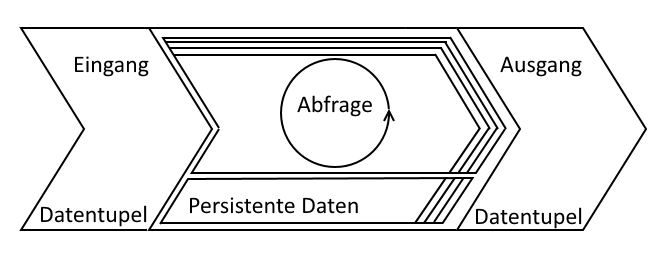
\includegraphics[width=1.0\textwidth]{bilder/StreamingFrameworkBasisModell.png}
\caption{Exemplarische Darstellung eines Basis Modells für Streaming frameworks
\label{fig:basismodell}}
\end{figure}

Dabei sind \textit{Input data streams} eine Sammlung von Werten und werden von \textit{Aurora} als eindeutiges Tupel mit einem Zeitstempel identifiziert. Innerhalb von \textit{Aurora} können mehrere \textit{Continous queries} gleichzeitig ausgeführt werden. Abbildung \ref{fig:basismodell} stellt in der Mitte der Grafik zwischen Eingang und Ausgang der Datentupel mehrschichtige Ebenen als Repräsentation für mehrere \textit{Continous queries} dar.

Ein \textit{Continous query} besteht aus \textit{boxes }und \textit{arrows}. \textit{Boxes} sind Operatoren um ankommende Datentupel in ausgehende Datentupel zu überführen. Durch die \textit{Arrows} wird eine Beziehung zwischen den \textit{Boxes} hergestellt. Ein komplexer Beziehungsgraph ist in eine Richtung gerichtet, es enthält keine Zyklen, hat mehrere Startknoten und einen Endknoten. Für die weitere Datenverarbeitung können in einem \textit{Continous query} zusätzlich persistente Datenquellen in einer \textit{Box} zur Transformation von Datentupeln hinzugefügt werden. Dazu wird in Abbildung \ref{fig:basismodell} unterhalb der \textit{Continous queries} ein mehrschichtiger separater Bereich für die persistenten Daten dargestellt. Im Endknoten des azyklisch gerichteten Graphen werden die transformierten Datentupel für weitere Anwendungen als Ausgabestrom von Datentupeln bereitgestellt. Die Abbildung \ref{fig:dag} stellt beispielhaft einen azyklisch gerichteten Graphen dar. Der dargestellte Graph enthält zwei Eingangsdatenquellen. Die obere Datenquelle wird zeitlich kurz vor dem Endknoten mit der unteren Datenquelle kombiniert. Die untere Datenquelle wird nach der zweiten Transformation in zwei neue Datenquellen aufgespalten. Nach drei Transformationen wird die mittlere Datenquelle in die oberer Datenquelle zeitlich an der sechsten Transformation überführt. Die untere Datenquelle wird mit der oberen Datenquelle an der siebten Transformation verbunden. Die letzte Transformation bildet den Endknoten.

\begin{figure}[htb!]
\centering
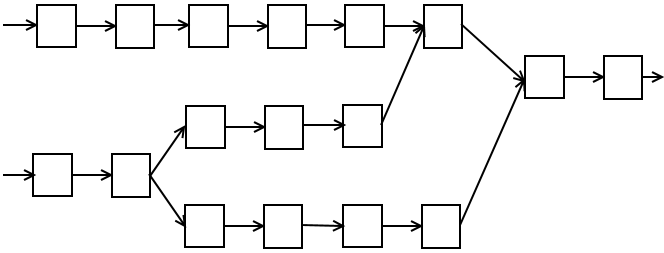
\includegraphics[width=1.0\textwidth]{bilder/DAG.png}
\caption{Darstellung eines azyklisch gerichteten Graphen
\label{fig:dag}}
\end{figure}

Das Datenmodell in \textit{Aurora} besteht aus einem \textit{Header}, dem Kopfbereich und Data, dem Datenteil als Tupel. Der Header in einem Basismodell besteht aus einem Zeitstempel. Mit dem Zeitstempel wird das Datenpaket eindeutig identifiziert und wird für das Monitoring in \gls{glo:qos} als einen Dienst für die Güte eingesetzt. Im Gegensatz zu \textit{Aurora} wird in der auf \textit{Aurora} basierten Weiterentwicklung \textit{Borealis} ein Vorhersagemodell für \gls{glo:qos} zu jedem Zeitpunkt in einem Datenfluss möglich. Dazu wird jedem Datentupel ein \gls{glo:vecme} hinzugefügt. Ein \gls{glo:vecme} besteht aus weiteren Eigenschaften wie zum Beispiel Ankunftszeit oder Signifikanz. In \citelit[S. 3, Kap. 2.4 QoS Model]{abadi2005design} werden \acrlong{glo:vecme} vorgestellt.

In \textit{Borealis} gibt es statuslose Operatoren und Operatoren mit einem Status. Statuslose Operatoren sind \textit{Filter}, \textit{Map} und \textit{Union}. Mit dem Filter kann eine Datenquelle nach bestimmten Bedingungen neue Datenquellen erzeugen. Der \textit{Map}-Operator kann bestimmte Datentupel in einer Datenquelle transformieren wie zum Beispiel durch anreichern von Informationen. Mit dem \textit{Union}-Operator können mehrere Datenquellen in eine Datenquelle zusammengeführt werden. Dazu wird ein Zwischenspeicher in der Größe \textit{n + 1} benutzt. In \citelit[S. 9, Abb. 3.1 Sample outputs from stateless operators]{borealis:programmer} wird eine Übersicht über die drei Operatoren \textit{Filter}, \textit{Map} und \textit{Union} anhand eines konkreten Beispiels dargestellt. Operatoren mit einem Status wie \textit{Join} und \textit{Aggregate} werden in \cite[S. 9, Kap. 3.2.2 Stateful Operators]{borealis:programmer} als Berechnungen von speziellen Zeitfenstern, dem \textit{window}, die mit der Zeit mitbewegen erläutert. In \cite[S. 10, Abb. 3.2 Sample output from an aggregate operator]{borealis:programmer} wird ein Schaubild zum Operator \textit{Aggregate} mit der Funktion \textit{group by}, \textit{average} und \textit{order} in einem \textit{window} gezeigt. Dabei werden eingehende Datenquellen mit einem Schema nach Zeit, Ort und Temperatur in einem Zeitfenster von einer Stunde gruppiert nach Raum, gemittelt nach Temperatur und sortiert nach Zeit in eine ausgehende Datenquelle transformiert. In Abbildung \ref{fig:querydiagramspe} wird ein Abfrage-Diagramm in einer \acrlong{glo:spe} dargestellt. Es werden zwei Sensoren S1 und S2 mit dem \textit{Union}-Operator in einen \textit{Stream} zusammengeführt. Der \textit{Stream} wird von zwei \textit{Aggregate}-Operatoren in einem Zeitfenster von 60 Sekunden getrennt und jeweils mit einem \textit{Filter}-Operator reduziert. Durch den \textit{Join}-Operator werden beide \textit{Streams} in einem Zeitfenster von 60 Sekunden zu einem dritten \textit{Stream} transformiert.

\begin{figure}[htb!]
\centering
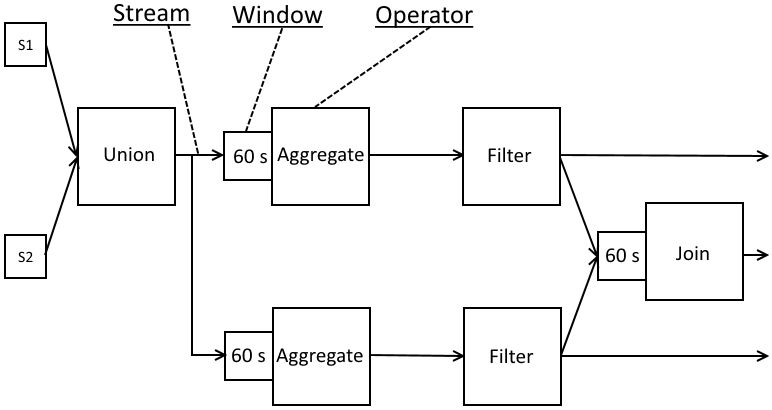
\includegraphics[width=1.0\textwidth]{bilder/QueryDiagram.png}
\caption{\acrlong{glo:spe}\label{fig:querydiagramspe}}
\end{figure}

Datentupel in \textit{Aurora} können aufgrund von technischen Fehlern, wie zum Beispiel Sensorausfall oder doppelter Parametrierung von mehreren Sensoren durch Hinzufügen, Löschen oder Aktualisieren verschiedene Versionen annehmen. Daher wurde das Datenmodell in \textit{Borealis} im \textit{Header} um einen Revisionstyp und einem Index erweitert. In separaten Speichern, den \glspl{glo:cp}, werden die Revisionen der Datentupel als Historie gehalten. Die \glspl{glo:cp} sind direkt an einer Datenquelle angeschlossen. Operatoren können auf die \glspl{glo:cp} durch die Identifikatoren im \textit{Header} auf benötigte Datentupel in der Historie zugreifen. 
%Push Vs Pull / Publisher-Subscriber Pattern / Software Design Pattern
%http://en.wikipedia.org/wiki/Push_technology#Long_polling

In den Streaming frameworks Storm, Kafka, Flume und S4 wird eine ähnliche Architektur wie sie im Referenzmodel von \textit{Aurora} und \textit{Borealis} vorgestellt wurde benutzt. Zwischen den Streaming frameworks gibt es dennoch Unterschiede. Das Referenzmodell von \textit{Aurora} und \textit{Borealis} soll dem Verständnis bei der Vorstellung der Streaming frameworks im Kapitel \ref{chapter:vorstellung} dienen und die Unterschiede aufzeigen. Mit der Einführung der Grundbegriffe und eines Referenzmodells soll nun das Kapitel \nameref{chapter:grundlagen} im Unterkapitel \ref{section:zusammenfassung} zusammengefasst werden.

\section{Zusammenfassung}
\label{section:zusammenfassung}

Im Kapitel \nameref{chapter:grundlagen} wurden die Streaming frameworks in die Bereiche der Informationsverarbeitung in verteilten Systemen, der Signaltheorie und der wiederkehrenden Berechnung von Daten in Datenströmen eingeordnet. Dabei wurden aktuelle Forschungsbereiche aufgezeigt und ein Referenzmodell als Grundlage dargestellt. In der Beschreibung des Referenzmodells sind die komplexen Operatoren und die Primitive vorgestellt worden. Ein Abfrage-Diagramm konnte anhand eines azyklisch gerichteten Graphen gezeigt werden. Mögliche Fehlererkennung durch Qualitätssicherungsmaßnahmen wurden durch \acrlong{glo:vecme} angesprochen. Fehlererkennungsmechanismen und Gütesicherung werden im Einzelnen im Kapitel \ref{chapter:vorstellung} aufgezeigt. Bevor die Streaming frameworks vorgestellt werden, wird in Kapitel \ref{chapter:kriterien} die Umgebung, der Markt, eine Studie, Kriterien für die Beurteilung der Streaming Frameworks vorgestellt und angewendet.
\chapter{Analyse}
\label{chapter:analyse}

In Kapitel \ref{chapter:grundlagen} wurden für die weitere Betrachtung der Streaming frameworks notwendige Grundbegriffe erläutert und ein Referenzmodell wie in Abbildung \ref{fig:basismodell} gezeigt vorgestellt. Zunächst wird der Markt anhand der Studie \citelit{studie:bidama} im Kontext von Big Data in dem Streaming frameworks zum Einsatz kommt vorgestellt. Die Studie \citelit{studie:bidama} wurde von Markl et al. im Auftrag des Bundesministeriums für Wirtschaft und Energie (BMWi) 2013 erstellt. 

\begin{quote}
Zentrales Ziel der vorliegenden Studie ist eine qualitative und quantitative Bewertung des Ist-Zustandes sowie der wirtschaftlichen Potenziale von neuen Technologien für das Management von Big Data. Daraus werden standortspezifische Chancen und Herausforderungen für Deutschland abgeleitet. In der Studie werden insbesondere auch rechtliche Rahmenbedingungen anhand von Einzelfällen betrachtet. Die Studie beinhaltet zudem konkrete Handlungsempfehlungen. 
\citelit[S. 3]{studie:bidama}
\end{quote}

Big Data wurde im Artikel \citelit{laney:threevs} von Laney 2001 in drei Dimensionen \textit{volume}, \textit{velocity} und \textit{variety} eingeordnet. Die Dimension \textit{volume} beschreibt den Umgang mit dem rasanten Anstieg an Datentransaktionen. \textit{Velocity} gibt die Geschwindigkeit an und \textit{variety} gibt die steigende Vielfalt der Daten an. In der Abbildung \ref{fig:bigdatacube} werden die drei Dimensionen in einem Würfel dem \textit{Big Data Cube} dargestellt. Die Abbildung \ref{fig:bigdatacube} wurde aus \citelit[S. 1, Abb. 1]{meijer2012your} in einfacher Form übernommen. So beschreibt Meijer \textit{volume} von klein \textit{small} nach groß \textit{big}, \textit{velocity} von ziehen \textit{pull} nach drücken \textit{push} und \textit{variety} von komplexen strukturierten Daten Fremd-/Primärschlüssel \textit{\acrshort{glo:fk}/\acrshort{glo:pk}} nach einfachen Zeigern auf Daten und Daten \textit{\acrshort{glo:k}/\acrshort{glo:v}}. Das herkömmliche relationale Datenbanksystem ist in der Abbildung \ref{fig:bigdatacube} unter den Koordinaten (\textit{small}, \textit{pull}, \textit{fk/pk}) zu finden. Unter den Koordinaten (\textit{small}, \textit{pull}, \textit{k/v}) wären Anwendungen zu finden, die das Konzept \textit{\gls{glo:orm}} implementieren. Beim Konzept \textit{\gls{glo:orm}} werden Objekte in relationalen Datenbanken abgebildet \citelit[S. 1]{meijer2012your}. Die Streaming frameworks werden unter den Koordinaten (\textit{big}, \textit{push}, \textit{fk/pk}) eingeordnet. Gegenüber den Streaming frameworks unter den Koordinaten (\textit{big}, \textit{pull}, \textit{fk/pk}) befinden sich die Batch Processing Engines, wie zum Beispiel Apache Hadoop \citeint{res:apache:hadoop}. In der unteren linken Ecke (big, pull, k/v) werden Lambda Ausdrücke eingeordnet. Lambda Ausdrücken werden anonyme Methoden möglich. Damit können einfache Abfragen auf Sammlungen formalisiert werden. Der Compiler erzeugt zur Laufzeit die Methoden im Hintergrund. In Java stehen die Lambda Ausdrücke erst ab Version 8 zur Verfügung \citeint{res:oracle:java8}.

\begin{figure}[htb!]
\centering
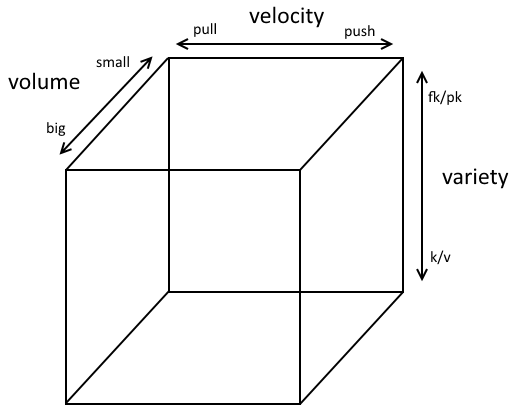
\includegraphics[width=1.0\textwidth]{bilder/bigdatacube.png}
\caption{Darstellung Big Data Cube
\label{fig:bigdatacube}}
\end{figure}

Relationale Datenbanksysteme stoßen im Zusammenhang der horizontalen Skalierung in der zentralisierten Systemarchitektur auf Probleme, wenn die Datenmenge die Kapazität einer Maschine übersteigt und dadurch das Ergebnis in keiner akzeptablen Zeit zurückgegeben wird \citelit[S. 30, Kap. 2.2.1]{edlich:nosql}. So zeigt Edlich et al. in dem Buch \citelit{edlich:nosql} einen alternativen Ansatz Daten zu halten. Dabei wird der Begriff \textit{NoSQL} als nicht relationales Datenbanksystem eingeführt und definiert \citelit[S. 2, K 1.2]{edlich:nosql}. In Verbindung mit horizontaler Skalierung, Replikation und niedriger Reaktionszeit wird in \citelit[S. 30, K. 2.2]{edlich:nosql} das \gls{glo:cap}-Theorem erklärt. Beim CAP-Theorem besteht der Konflikt in der Konsistenz \textit{C}. Es gilt zu Entscheiden ob die Konsistenz gelockert wird oder nicht. Bei einer lockeren Konsistenz und damit einer hohen Verfügbarkeit und Ausfalltoleranz können in einem Verbindungsausfall alte Zustände zurückgegeben werden. Falls nicht gelockert wird kann der Umstand in Kraft treten, sehr lange Reaktionszeiten zu erhalten. %Out-of-order, Dropped, Duplicate Messages
Daher wurde das Konsistenzmodell \gls{glo:base} eingeführt. Es basiert auf einem optimistischen Ansatz. Eine Transaktion nimmt den Status konsistent nicht unmittelbar ein. Erst nach einer gewissen Zeitspanne ist die Transaktion konsistent. Dieses Verhalten wird als \textit{Eventually Consistancy} bezeichnet. Als Beispiel gibt Edlich et al. in \citelit[S. 33, K. 2.2.3]{edlich:nosql} replizierende Knoten in einer Systemarchitektur an. 
% 3V Darstellung, nächere Darstellung ACID(::CAP)->BASE %% --> CRDTs

So wurden in der Studie \citelit{studie:bidama} neben der Einführung in Big Data, Stärken, Schwächen, Chancen und Risiken für die Branchen Handel, Banken, Energie, Dienstleistungen, Öffentlicher Sektor, Industrie, Gesundheitssektor, Marktforschung, Mobilitätsleistungen, Energie und Versicherungen als tabellarische Übersicht in \citelit[S. 105, Tab. 18]{studie:bidama} ausgegeben. In \citelit[S. 107, Abb. 54]{studie:bidama} werden Branchenschwerpunkte abgeleitet. Die genannte Abbildung wird im folgenden Zitat textuell erneut wiedergegeben:

\begin{quote}
	\begin{enumerate}
		\item Entwicklung neuartiger Technologien, um eine skalierbare Verarbeitung von komplexen Datenanalyseverfahren auf riesigen, heterogenen Datenmengen mit hoher Datenrate zu realisieren
		\item Senkung der Zeit und Kosten der Datenanalyse durch automatische Parallelisierung und Optimierung von deklarativen Datenanalysespezifikationen
		\item Schaffung von Technologieimpulsen, die zur erfolgreichen weltweiten Kommerzialisierung von in Deutschland entwickelten, skalierbaren Datenanalysesystemen führen
		\item Ausbildung von Multiplikatoren im Bereich der Datenanalyse und der skalierbaren Datenverarbeitung, welche die Möglichkeiten von Big Data in Wissenschaft und Wirtschaft tragen werden
		\item Technologietransfer an Pilotanwendungen in Wissenschaft und Wirtschaft
		\item Schaffung eines Innovationsklimas durch Konzentration von kritischem Big Data Know-how, damit deutsche Unternehmen und Wissenschaft nicht im Schatten des Silicon Valleys stehen
		\item Interaktive, iterative Informationsanalyse für Text und Weiterentwicklung geeigneter Geschäftsmodelle zur Schaffung von Marktplätzen für Daten, Datenqualität und Verwertung von Daten
		\item Datenschutz und Datensicherheit
	\end{enumerate}
	\citelit[S. 107, Abb. 54]{studie:bidama}
\end{quote}

Aus den abgeleiteten Schwerpunkten können mehrere Kriterien für die Betrachtung der Streaming frameworks in Kapitel \ref{chapter:vorstellung} und des Referenzmodells in Kapitel \ref{section:technologie} herangezogen werden. Zunächst werden die gewonnen Kriterien in einer Liste aufgezählt. Anschließend werden die einzelnen Kriterien als Bewertungskriterien für die weitere Untersuchung der Streaming frameworks definiert. Daraufhin werden die Bewertungskriterien auf das Referenzmodell angewendet.

\begin{itemlist}{Bewertungskriterien}{liste:bewkrit}
	\item Architektur
	\item Prozesse und Threads
	\item Kommunikation
	\item Namenssystem
	\item Synchronisierung
	\item Pipelining und Materialisierung
	\item Konsistenz und Replikation	
	\item Fehlertoleranz
	\item Sicherheit	
	\item Erweiterung
	\item Qualität
\end{itemlist}

Die ermittelten Bewertungskriterien aus Liste \ref{liste:bewkrit} unterstützen die Feststellung eines Streaming frameworks und des Referenzmodells. Damit die einzelnen Bewertungskriterien bei der Anwendung eindeutig und klar sind, werden diese zunächst definiert und zusätzlich erläutert.

\begin{description}
	\item[Architektur] stellt den verwendeten Architekturstil vor und ordnet in eine Systemarchitektur ein.
	\item[Prozesse und Threads] zeigen die Anwendung von blockierendem oder nicht blockierendem Zugriff, also einer Verbindung zwischen Client und einem Server. Während der Betrachtung wird der Einsatz der verteilten Verarbeitung in der eingesetzten Architektur geprüft.
	\item[Kommunikation] gibt die Form des Nachrichtenaustauschs zwischen Client und Servern an. Zum Austausch der Nachrichten kommen Nachrichtenprotokolle zum Einsatz. Dabei wird auf die Protokollschicht \textit{Middleware}-Protokoll eingegangen. Im \acrshort{glo:osi}-Modell entspricht die Sitzungs- und Darstellungsschicht einer \textit{Middleware}-Schicht \citelit[S. 148, Abb. 4.3 angepasstes Referenzmodell]{tanenbaum:vs}. Dabei werden unterschiedliche Strategien \gls{glo:rpc}, Warteschlangensysteme, Kontinuierliche Systeme und Multicast Systeme, die beim Nachrichtenaustauschs eingesetzt werden, innerhalb der \textit{Middleware}-Protokolle eingeordnet. Außerdem wird das Verbindungsmodell, die Nachrichtenstruktur und der Einsatz einer Protokollversionierung vorgestellt. Weiterhin wird die Unterstützung von unterschiedlichen Nachrichtenkodierungen und Statusverwaltung betrachtet.
	\item[Namenssystem] zeichnet den Ansatz eines Benennungssystems. Hierbei wird linear-, hierarchisch- oder attributbasiert klassifiziert.
	\item[Synchronisierung] beschreibt die verwendeten Algorithmenarten. 
	\item[Pipelining und Materialisierung] gibt eine Technik an, ob komplexe Aggregate berechnet werden und innerhalb der Abfragen wieder benutzt werden können.
	\item[Konsistenz und Replikation] zeigt die Skalierungstechnik auf und stellt die Verwaltung der Replikation vor. 	
	\item[Fehlertoleranz] zeigt das verwendete Fehlermodell und stellt eine Strategie im Wiederherstellungsfall vor.
	\item[Sicherheit] stellt das Konzept vor und beschreibt den Einsatz von sicheren Kanälen und der Zugriffssteuerung.	
	\item[Erweiterung] beschreibt Methoden weitere Systemarchitekturen anzuschließen.
	\item[Qualität] zeigt das verwendete Modell für die Dienstgüte.
\end{description}

In der Liste \ref{liste:bewkrit} wurden Bewertungskriterien vorgestellt und definiert, die nun auf das Referenzmodell aus Kapitel \ref{section:technologie} angewendet werden. In der Tabelle \ref{tab:bewrefaurbor} wird eine Übersicht über die Bewertung zum Referenzmodell Aurora Borealis gegeben. Als Architektur wird strukturierte Peer-to-Peer-Architektur angegeben. In einer dezentralisierten Architektur, wie es die strukturierte Peer-to-Peer-Architektur ist, werden Nachrichten zwischen den Rechnerknoten die auch Peers genannt werden, mit Hilfe von verteilten Hashtabellen ausgetauscht. Dabei übernimmt bei Aurora Borealis ein Knoten den Master bei dem Nachrichten von den Verarbeitungsknoten zurückkommen. So wird in Abbildung \ref{fig:aurborinaction} eine Anwendung gezeigt in der ein Server 1 die Datenverarbeitung auf zwei Datenverarbeitungsservern 2 und 3 ausführen lässt und das Ergebnis aus der Daten- und Verarbeitungsebene an einen Rechner 4 mit der Benutzerschnittstelle zurückschickt. \citelit[S. 64, Kap. 2.2.2]{tanenbaum:vs} 

Aus der strukturierten Architektur folgt die Frage wie Prozesse untereinander kommunizieren. Die Prozesse kommunizieren entweder lokal oder entfernt asynchron über \gls{glo:rpc}. Anfragen von entfernten Prozessen werden automatisch lokal übersetzt. Ein Rechnerknoten stellt damit eine vollständige Verarbeitungseinheit dar. Der Prozess muss also gleichzeitig als Client und als Server arbeiten und ist dadurch symmetrisch. \citelit[S. 6, Kap. 2]{borealis:developer}

\begin{table}[htbp]
	\centering
		\begin{tabular}{@{}ll@{}} \toprule
			\textbf{Kriterium} & \textbf{Bewertung} \\ \midrule
			Architektur & Strukturierte Peer-to-Peer-Architektur \\
			Prozesse und Threads & Interaktion symmetrisch \\ 
			Kommunikation &  Transportunabhängiges \gls{glo:rpc}\\
			Namenssystem &  Attributbasierte Benennung\\
			Synchronisierung &  Zentralisierter Algorithmus \\
			Pipelining und Materialisierung &  In/Out Attribut\\
			Konsistenz und Replikation & Push-basiertes Monitoring \\			
			Fehlertoleranz &  Replikation \\
			Sicherheit & Nur Verfügbarkeitsprüfung \\			
			Erweiterung & Nur Eigenentwicklung \\
			Qualität &  Monitor, Optimierer, Voruasberechnen, Lokal und Global\\
			\bottomrule			
		\end{tabular}
	\caption{Bewertung Referenzmodell Aurora Borealis}
	\label{tab:bewrefaurbor}
\end{table}

In der Kommunikation wird ein transportunabhängiges \gls{glo:rpc} angegeben \citelit[S. 7, Abb. 2.1]{borealis:developer}. So findet der Nachrichtenaustausch zwischen zwei entfernten Rechnern asynchron statt. Die entfernten Rechner entsprechen den Verarbeitungseinheiten. Zwischen einem führenden Rechner und einem entfernten Rechner werden zwei Nachrichten verschickt. Die erste Nachricht führt eine Aktion auf dem entfernten Rechner aus und die zweite Nachricht ist das Ergebnis das vom entfernten Rechner dem führenden Rechner zurück gegeben wird. Hierbei beschreibt Tanenbaum et al. in \citelit[S. 158, Kap. 4.2.3]{tanenbaum:vs} den Nachrichtenaustausch als verzögerter synchroner \gls{glo:rpc}. Das kontinuierliche Verarbeiten von Abfragen wird dabei von einem führenden Rechner der \textit{Middleware}-Schicht übernommen. Dem führenden Rechner dem \textit{Global Load Manager} \citelit[S. 28, Kap. 5]{borealis:developer} wird beim Start des Systems eine \textit{Topology} übergeben. Die \textit{Topology} enthält einen Ausführungsplan mit komplexen Abfragen. Der \textit{Global Load Manager} verwaltet die Auslastung der entfernten Rechner und gleicht hohe Last durch Umverteilung der Aufgaben auf andere Rechner aus. Jeder Verarbeitungseinheit besteht aus einem \textit{Availabilty Monitor} \citelit[S. 38, Abb. 7.2]{borealis:developer} dem Verfügbarkeitsmonitor, einem \textit{Load Manager} der mit dem \textit{Global Load Manager} kommuniziert und einem \textit{QueryProcessor} der die Abfrage ausführt \citelit[S. 10, Kap 3.2]{borealis:developer}. 

Bei der Anwendung einer Verarbeitung in Aurora Borealis wird eine Konfiguration in einer \gls{glo:xml}-Datei für die Verteilung der Abfragen benötigt. Im Quelltext \ref{lst:aurorborealisdeoployconf} wird eine Konfiguration für Zwei Verarbeitungseinheiten formuliert. Einer Verarbeitungseinheit wird die Abfrage \textit{mycount} und der anderen Verarbeitungseinheit die Abfrage \textit{myfilter} zugeordnet. Beide Verarbeitungseinheiten abonnieren den Eingangsstrom \textit{stream} \textit{Aggregate} und veröffentlichen den \textit{stream} \textit{Packet} an die angegebene Verteilungseinheit. Für die Abfrage wird eine zustäzlich \gls{glo:xml}-Datei verwendet. In der Konfiguration \ref{lst:aurorborealisqueryconf} werden die Abfragen \textit{mycount} und \textit{myfilter} für die Zwei Verarbeitungseinheiten definiert. Die Abfrage wird im XML-Tag \textit{borealis} ausgezeichnet. Mit dem XML-Tag \textit{schema} werden komplexe Aurora Borealis Datentypen definiert. 

Die Benennung wird durch Attribute gekennzeichnet. Zum Beispiel hat das Schema \textit{PacketTuple} ein Feld mit dem Namen \textit{time} und den primitiven Datentypen \textit{int} in \gls{glo:coo}. Es werden Sechs Feldtypen (\textit{int}, \textit{long}, \textit{single}, \textit{double}, \textit{string}, \textit{timestamp}) unterstützt \citelit[S. 17, Tab. 4.2]{borealis:programmer}. Borealis erzeugt durch die \textit{Marshalling}-Anwendung eine \gls{glo:coo}-Struktur \textit{struct} vom Typ \textit{TupleHeader} \citelit[S. 37, Kap. 5.2.1]{borealis:programmer}. Die \textit{Marshalling}-Anwendung kapselt die komplexe auf \textit{Borealis} spezialisierte \gls{glo:nmstl} für \gls{glo:coo} \citelit[S. 35, Kap. 5.2]{borealis:programmer}. Der Quelltext \ref{lst:aurorborealismytest} zeigt die Methoden der \textit{Marshalling}-Anwendung für die beschriebenen Konfigurationen \ref{lst:aurorborealisdeoployconf} und \ref{lst:aurorborealisqueryconf}. In der Abfrage der ersten Verarbeitungseinheit wird im \gls{glo:xml}-Tag \textit{parameter} mit die Aggregatsfunktion \textit{count()} die Anzahl der Pakete jede Sekunde nach Zeit sortiert. Die Tabelle in \citelit[S. 23, Tab. 4.5]{borealis:programmer} zeigt eine Übersicht über die möglichen Aggregat-Parameter. Die zweite Abfrage filtert den Ausgabestrom aus der ersten Abfrage nach geraden Zeitwerten und gibt den Ausgabestrom \textit{Aggregate} zurück. Die Abbildung \ref{fig:aurborinaction} zeigt die Ausführung der Kommunikation.

\begin{figure}[htb!]
\centering
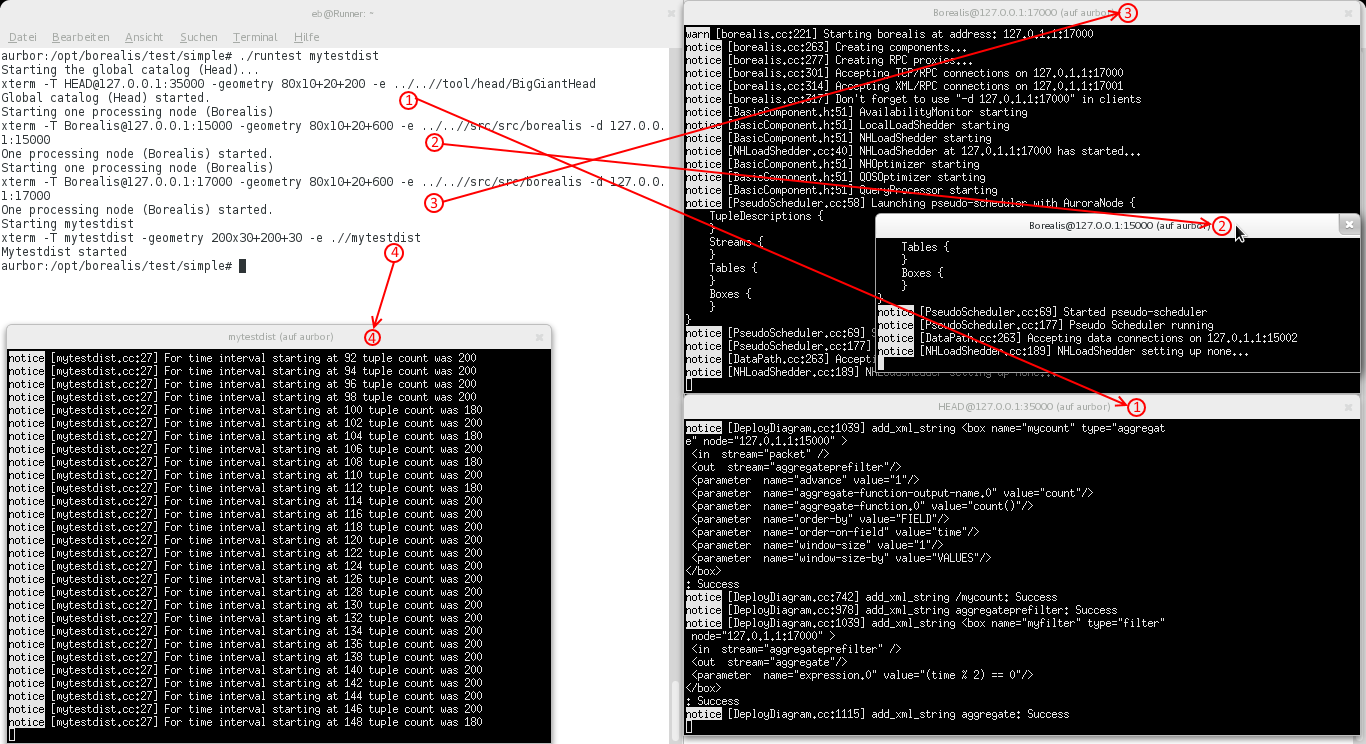
\includegraphics[width=1.0\textwidth]{bilder/auroraborealisinaction.png}
\caption{Aurora Borealis mit einem Master zwei Servern und einem Konsumenten
\label{fig:aurborinaction}}
\end{figure}

Pipelining wird durch den Einsatz von Eingangs- und Ausgangsstrom in Abfragen erreicht. In der Konfiguration \ref{lst:aurorborealisqueryconf} wird von der ersten Einheit ein spezialisiertes Datentupel \textit{AggregatePreFilter} erzeugt und die zweite Einheit bezieht das Ergebnis und verändert es. Zusätzlich können über eine \textit{Map}-Funktion in der Abfrage mehrere Datenströme erzeugt und komplex verarbeitet werden \citelit[S. 20, Kap. 4.9.1]{borealis:programmer}.

Die Konsistenz in den Verarbeitungseinheiten wird mit dem \textit{Consistancy Manager} erreicht. Durch die zusätzliche Komponente \textit{Availability Monitor} werden Statusinformation zwischen den Einheiten ausgetauscht. Einzelne Verarbeitungseinheiten können repliziert werden. Die Konfiguration der Replikation wird in der Konfiguration \ref{lst:aurorborealisdeoployconf} hinzugefügt. Im Gegensatz zum \gls{glo:xml}-Tag \textit{box} wird bei der Replikation \textit{replica\_set} verwendet. Die Abfrage wird ebenfalls dem \textit{replica\_set} zugeordnet. Innerhalb des \textit{replica\_set} werden einzelne \textit{node}-Elemente mit Zieladresse hinterlegt. Durch die Replikation wird in Aurora Borealis Fehlertoleranz erreicht. \citelit[S. 34, Kap. 7]{borealis:developer}

In der Sicherheit werden keine Sicherheitsrichtlinien vorgestellt und angewendet. Die Kommunikation zwischen einzelnen Rechnern findet unverschlüsselt auf TCP-Ebene über RPC statt. Eine Authentifizierung und Autorisierung wird nicht durchgeführt. Eine leichtgewichtichtete Kontrolle kann durch den \textit{Consistancy Manager} und dem \textit{Availability Monitoring} als Protokollwerkzeuge angesehen werden. Für komplexe Kontrollen ist eine eigene Implementierung notwendig \citelit[S. 38, Kap. 7.2.2]{borealis:developer}.

Erweiterungen können durch eigene Entwicklung in den bestehende Quelltext hinzugefügt werden. Methoden für weitreichende Abfragen in andere Umgebungen wie zum Beispiel Python sind nicht vorhanden. Eine umfangreiche Testabdeckung und eine gute Dokumentation für bestehende Methoden sind vorhanden. Das Erstellen von Aurora Borealis wurde bisher nur auf einer älteren Linux-Distribution durchgeführt. Der Quelltext in der letzten Version 2.8 ist auf den Linux Compiler Version 3.1.1 angepasst und muss beim Einsatz der aktuellen Compiler-Version aktualisiert werden. Im Anhang \ref{sec:aurborinstall} wird eine ausführliche Anleitung zur Installation von Aurora Borealis in der aktuellen Version 2.8 mit einer älteren Debian-Distribution vorgestellt. Der Quelltext von Aurora Borealis und die verwendete Debian-Version liegt im Verzeichnis \textit{anhangSoftwareZusatz} bei. Eine lauffähige virtuelle Maschine steht ebenfalls im gleichen Verzeichnis bereit.

Die Qualität der Dienste wird in Aurora Borealis durch verschiedene Mechanismen erreicht. Lokal werden pro Rechnereinheit mit dem \textit{Local Monitor} Statuswerte von \gls{glo:cpu}, Festplatte, Bandbreite und Energieversorgung erfasst und an den globalen \textit{End-point Monitor }übertragen. Der \textit{End-point Monitor} wertet die Qualität des Dienstes aus und führt eine Statistik pro Erfassung. Optimiert wird lokal durch den \textit{Local Monitor} mit dem \textit{Local} und \textit{Neighborhood Optimizer} und global durch den \textit{Global Optimizer}. Probleme werden durch die Monitore erkannt. Da jedem Datentupel ein \textit{Vector of Metrics} dazugeschaltet ist und es möglich ist zusätzlich einen \textit{Vector of Weights} (Lifetime, Coverage, Throughput, Latency) dazuzuschalten, ist eine Berechnung der Ursache eines \gls{glo:qos}-Problems möglich. \citelit[S. 7, Kap. 5]{abadi2005design}

In der Analyse wurden die Vier Vs in \textit{Big Data} vorgestellt und die Streaming frameworks wurden darin in einem Vergleich zu relationalen Datenbanksystemen eingeordnet. Weiterhin wurden die Konsistenz und die Verfügbarkeit im Zusammenhang von CAP und BASE vorgestellt. Mit der Studie \citelit{studie:bidama} und \citelit{tanenbaum:vs} wurden Bewertungkriterien in der Liste \ref{liste:bewkrit} erarbeitet. Abschließend wurde ausgehend von den Bewertungskriterien das Referenzmodell Aurora Borealis ausgewertet. In Kapitel \ref{chapter:vorstellung} werden nun die Streaming frameworks vorgestellt und mit Bewertungskriterien in Liste \ref{liste:bewkrit} ausgewertet.
\chapter{Vorstellung Streaming Frameworks}
\label{chapter:vorstellung}

In Kapitel \ref{chapter:grundlagen} und \ref{chapter:analyse} wurden Grundlagen geschaffen, eine Analyse durchgeführt und ein Referenzmodell mit Bewertungskriterien vorgestellt und für die Anwendung auf die Streaming frameworks erläutert. In den folgenden Unterkapitel werden die einzelnen Streaming frameworks Apache Storm, Apache Kafka, Apache Flume und Apache S4 vorgestellt. Jedes Unterkapitel beginnt zuerst mit einer Übersicht über das Streaming framework. Anschließend wird kurz auf die Entstehung des Streaming frameworks bis zum Zeitpunkt der Erstellung dieser Thesis eingegangen. Nach der kurzen Übersicht werden die Bewertungskriterien aus Liste \ref{liste:bewkrit} auf das Streaming framework angewendet. Dabei wird wie in der Analyse des Referenzmodells vorgegangen. Eine kurzer Vergleich zwischen dem Referenzmodell wird am Ende des Unterkapitels eines Streaming frameworks durchgeführt.

\section{Apache Storm}
\label{section:storm}

Apache Storm wird vom Hauptentwickler Nathan Marz im Proposal als verteiltes, fehlertolerantes und hochperformantes Echtzeitberechnungssystem definiert. Ursprünglich wurde die Anwendung von der Firma Backtype in 2011 entwickelt. Im gleichen Jahr wurde die Firma Backtype von Twitter übernommen und der Quelltext auf Github \citeint{GitHub} unter dem Repository \textit{storm} \citeint{storm:GitHub} von Nathan Marz veröffentlicht. In 2013 wurde die Aufnahme von Storm in die \gls{glo:asf} geplant. Dazu wurde ein Storm Proposal von Nathan Marz eingereicht. \citeint{storm:apache:stormProposal} 

Seit 2013 befindet sich Storm im Apache Incubation-Prozess \citeint{storm:apache:stormIncubationStatus}. Eine Überführungsversion 0.9.1-incubating wurde dafür eingerichtet. Der Quelltext und das Lizenzmodell wird in die \gls{glo:asf} aufgenommen \citeint{apache:softwareFoundation}. Der Verlauf des Überführungsprozesses zur \gls{glo:asf} wird auf der Incubator-Statusseite \citeint{storm:IncubatorStatusPage} festgehalten. In der Tabelle \ref{tab:vorstorm} wird eine Kurzübersicht über Apache Storm gegeben. Darin wird ein aktiver Entwicklungsstatus angegeben. Die Aktivität wird aus dem GitHub \textit{Contributors-Graph} bei 84 Projektteilnehmern bestimmt \citeint{storm:Contributors}. Zur Entwicklung werden mehrere Sprachen Clojure, Java und Python angegeben. Nathan Marz gibt an Storm in der Programmiersprache Clojure \citeint{clojure} zu entwickeln und mit Java  \citeint{javaAbout} kompatibel zu sein, neben Java und Clojure  findet die Github Sprachen-Suche \citeint{storm:GitHubApacheMirror} im Repository \textit{storm} auch Python \citeint{pythonAbout}. Ab Version 0.9.1-incubating wird eine verbesserte Plattformkompatibilität zum Betriebssystem Microsoft Windows angeboten und die Standardtransportschicht ZeroMq \citeint{zeromq:guide} wurde durch Netty \citeint{netty} ersetzt \citeint{storm:Changelog}.

\begin{table}[htbp]
	\centering
		\begin{tabular}{@{}ll@{}} \toprule
			\textbf{Faktum} & \textbf{Beschreibung} \\ \midrule
			Hauptentwickler & Nathan Marz \\
			Stabile Version & 0.9.1-incubating vom 22.02.2014 \\ 
			Entwicklungsstatus &  Aktiv \\
			Entwicklungsversion & 0.9.2-incubating, 0.9.3-incubating \\
			Sprache & Clojure, Java, Python \\
			Betriebssystem & Platformübergreifend (Microsoft Windows mit Cygwin Umgebung) \\
			Lizenz & Eclipse Public License 1.0 (Incubating Apache License version 2.0) \\
			Webseite &  \citeint{storm:home} \\
			Quelltext & \citeint{storm:GitHubApacheMirror} \\			
			\bottomrule			
		\end{tabular}
	\caption{Kurzübersicht Apache Storm}
	\label{tab:vorstorm}
\end{table}

In Tabelle \ref{tab:bewstorm} werden die Bewertungskriterien aus Kapitel \ref{chapter:kriterien} in Apache Storm geprüft. Als Architektur wird die moderne Systemarchitektur Strukturierte Peer-To-Peer-Architektur, die eine horizontale Verteilung unterstützt, angegeben. Apache Storm besteht aus drei Komponenten: \textit{Nimbus}, \textit{Supervisor} und \textit{UI}. Der \textit{Nimbus} stellt die zentrale Stelle und übernimmt die Aufgabe des \textit{Scheduler} - einem Arbeitsplaner. Der \textit{Nimbus} is klein gehalten und verteilt die Aufgaben zwischen den Arbeitsknoten. Die Arbeitsknoten werden in Apache Storm \textit{Supervisor} genannt. Mehrere Supervisor-Instanzen sind in einem Apache Storm Cluster möglich. Die dritte Komponente \textit{UI} visualisiert den momentanen Status der Apache Storm Komponenten \textit{Nimbus} und \textit{Supervisor}. 

Bei der Verarbeitung von Informationen kann in Apache Storm pro Verarbeitungseinheit die Anzahl an benötigten Threads als Argument explizit übergeben werden. Die Konfiguration dazu findet im Quelltext statt. Um eine komplexe Verarbeitung durchzuführen, muss in Apache Storm eine \textit{Topology} implementiert und veröffentlicht werden. Die \textit{Topology} wird auf dem Apache Storm Cluster permanent ausgeführt und kann nicht dynamisch verändert werden. Die Kommunikation erfolgt zwischen den einzelnen Apache Storm Komponenten mit einem zusätzlichen Werkzeug: Apache ZooKeeper \citeint{zookeeper:Home}. Apache ZooKeeper wird als verteilte Synchronisation und Koordination der Aufgaben durch Nimbus auf tieferer Ebene verwendet. Auf der Transportebene kommunizieren Verarbeitungseinheiten durch das asynchrone Client-Server-Framework Netty \citeint{netty}.

Eine komplexe Verarbeitung bzw. Abfrage in einer \textit{Topology} besteht aus \textit{Spouts} und \textit{Bolts}. Die Kommunikation ist dabei einseitig. Ein Empfänger-\textit{Bolt} kann keine Nachricht an einen Sender-\textit{Bolt} zurück schicken. Mit einem \textit{Spout} wird eine externe Datenquelle beschrieben und ein \textit{Spout} liefert eine permanente Folge von ungebunden Tupeln. Ein Tupel ist die Hauptdatenstruktur und kann unterschiedliche Datentypen (integers, longs, shorts, bytes, strings, doubles, floats, booleans und selbstentwickelte) enthalten. Die Folge von ungebundenen Tupeln wird in Apache Storm als \textit{Stream} bezeichnet. Um einen \textit{Spout} zu implementieren reicht es die Schnittstelle \textit{IRichSpout} zu implementieren oder die Klasse \textit{BaseRichSpout} zu erweitern. 

Bei einer Erweiterung von \textit{BaseRichSpout} sind mindestens die Methodenamen \textit{open}, \textit{nextTuple} und \textit{declareOutputFields} zu implementieren. In der Methode \textit{open} kann zum Beispiel eine interne Liste über einen Java-Listener bei einem Dateneingang in einem Datenadapter gefüllt werden. Die Methode \textit{nextTuple} wird jede erste Millisekunde ausgeführt und wenn Nachrichten in der Liste enthalten sind, kann der \textit{SpoutOutputCollector} einen Stream mit einer eindeutigen StreamId und einem Tuple aussenden. Wenn die Nachricht nicht vollständig übertragen wurde, wird über ein \textit{Callback-Methode} \textit{ack} oder \textit{fail} in der implementierten Klasse \textit{Spout} zurückgegeben. Damit wird in Apache Storm sichergestellt, dass die Nachricht mindestens einmal vollständig verarbeitet wurde \citeint{storm:SpoutOutputCollector}. In der Methode \textit{declareOutputFields} wird die Felddefinition der Ausgabe für die weitere Verarbeitung angegeben. \citeint{storm:Spout}

Ein \textit{Bolt} nimmt ein Tupel auf und gibt Tupel wieder aus. Innerhalb eines \textit{Bolt} können Tupel verändert werden. Nachdem Start der \textit{Topology} wird ein \textit{Bolt} erst auf den \textit{Supervisor} übertragen und deserialisiert. \textit{Nimbus} ruft auf der Instanz anschließend die Methode \textit{prepare} auf. In Java muss für die Implementierung eines \textit{Bolt} die Schnittstelle \textit{IBolt} oder \textit{IRichBolt} implementiert werden. Alternativ können auch Basisimplementierungen verwendet werden, wie zum Beispiel \textit{BaseBasicBolt} oder \textit{BaseRichBolt}. Mit der Methode \textit{execute} werden die Tupel angepasst und über den \textit{OutputCollector} ausgesendet. Apache Storm erwartet beim Eingang eines Tupels in einem \textit{Bolt} Bestätigung über die Methode \textit{ack} oder \textit{fail}. Andernfalls kann Apache Storm nicht feststellen, ob eine Nachricht vollständig verarbeitet wurde. \citeint{storm:Bolt}

\begin{figure}[htb!]
\centering
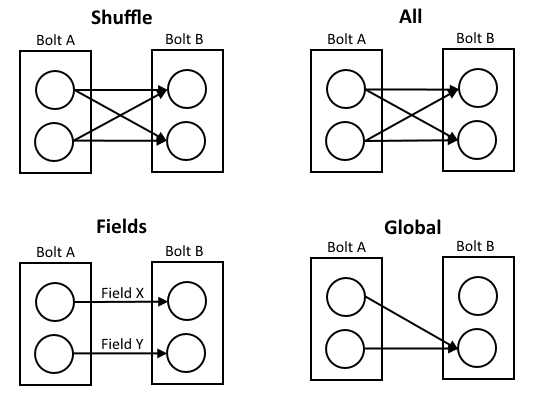
\includegraphics[width=1.0\textwidth]{bilder/stormGroupings.png}
\caption{Apache Storm Gruppierungen
\label{fig:stormGroupings}}
\end{figure}

Durch den \textit{TopologyBuilder} kann eine komplexe Abfrage aus \textit{Spouts} und \textit{Bolts} zusammengesetzt werden. Der \textit{TopologyBuilder} stellt dazu \textit{set}-Methoden für \textit{Spouts} und \textit{Bolts} bereit. Bei dem Setzen eines \textit{Spout} oder eines \textit{Bolt} muss immer eine Referenz-Identifikationsnummer angegeben werden. Durch die Referenz können \textit{Bolt}- oder \textit{Spout}-Komponenten untereinander verbunden werden. Weiterhin kann mit dem Argument \textit{parallelism\_hint} die Anzahl der \textit{Tasks} eingestellt werden, die zur Ausführung benutzt werden. Jeder \textit{Task} wird im Storm Cluster auf einem eigenen \textit{Thread} ausgeführt. Wenn die \textit{setBolt}-Methode aufgerufen wird, wird ein Objekt \textit{InputDeclarer} erzeugt. Darin können verschiedene Gruppierungen (\textit{Shuffle}, \textit{Fields}, \textit{All}, \textit{Global}, \textit{None}, \textit{Direct}, \textit{LocalOrShuffle} \citeint{storm:InputDeclarer}) angegeben werden, um den Stream in definierte Teile zu trennen. In Abbilung \ref{fig:stormGroupings} werden Vier Standardgruppierungen in Apache Storm gezeigt. Mit einem \textit{ShuffleGrouping} werden Tupel eines \textit{Stream} zufällig über die \textit{Tasks} verteilt. Beim \textit{FieldsGrouping} wird der \textit{Stream} durch die Angabe eine Schlagworts getrennt. Tupel mit dem gleichen Schlagwort werden immer an den gleichen \textit{Task} gesendet. Das \textit{AllGrouping} wird auf allen Tasks des \textit{Bolt} repliziert und beim \textit{GlobalGrouping} wird der \textit{Stream} zu einem \textit{Task} gesendet. Weiterhin gibt es noch das \textit{NoneGrouping} bei dem der \textit{Stream} auf dem gleichen \textit{Task} ausgeführt wird und beim \textit{DirectGrouping} entscheidet der \textit{Stream}-Erzeuger auf welchen Konsumenten-\textit{Task} der \textit{Stream} gesendet wird. Durch die Schnittstelle \textit{CustomStreamGrouping} is eine weitere konkrete Implementierung für eine \textit{Grouping}-Strategie möglich. \citeint{storm:TopologyBuilder}

In Apache Storm wird eine Abstraktion \textit{Trident} für eine transaktionsorientierte Abfrage- und Datenverarbeitung bereitgestellt. Mit \textit{Trident} ist es möglich eine Stapelverarbeitung mit Statusinformationen durchzuführen. Es gibt Fünf Ausführungstypen: \textit{Partition-local}, \textit{Repartitioning}, \textit{Aggregation}, \textit{GroupedStreams} und \textit{Merges and Joins}. In \citeint{storm:Trident} wird \textit{Trident} näher erläutert. In den folgenden Absätzen wird kurz auf die möglichen Funktionen mit \textit{Trident} aus \citeint{storm:Trident} eingegangen.

Unter \textit{Partition-local} werden Operatoren (\textit{function}, \textit{filter}, \textit{partitionAggregate}, \textit{partitionPersist}, \textit{projection}) lokal in einem Stapelelement ausgeführt. Die Operatoren \textit{function} und \textit{filter} erben jeweils von der gleichen Basisklasse \textit{BaseFunction}. Bei den Methoden \textit{partitionAggregate} und \textit{partitionPersists} können unterschiedliche Strategien entwickelt werden. Ein neues Aggregat kann mit der \textit{Aggregator}-Schnittstelle oder den erweiterten Schnittstellen \textit{CombinerAggregator} oder \textit{ReducerAggregator} implementiert werden. Um nicht im bestehenden Arbeitsspeicher mit der \textit{MemoryMapState.Factory()} Daten zu speichern, kann über eine konkrete Implementierung der Schnittstelle \textit{IBackingMap} eine neue Strategie zur Datenablage erzeugt werden. Mit \textit{Projection} können Teile der Felder aus einem \textit{Stream} in einem neuen \textit{Stream} unverändert abgebildet werden.

Beim \textit{Repartitioning} kann die Stapelverarbeitung durch \textit{Repartitioning}-Funktionen (\textit{shuffle}, \textit{broadcast}, \textit{partitionBy}, \textit{global}, \textit{batchGlobal}, \textit{partition}) geändert bzw. neu strukturiert werden. Zum Beispiel kann sich die Anzahl der \textit{Tasks} zur parallelen Datenverarbeitung ändern. Mit dem \textit{Repartitioning} ist es möglich die \textit{Tasks} im Cluster neu zu verteilen. Die Methode \textit{groupBy} nutzt \textit{Repartitioning} um den \textit{Stream} mit \textit{partitionBy} neu zu strukturieren. Gruppierte und aggregierte \textit{Streams} können mit bestehenden Apache Storm Primitiven verkettet werden.

\textit{Streams} können in \textit{Trident} durch die spezielle \textit{TridentTopology} zusammengeführt werden. Die \textit{TridentTopology} bietet dazu die Methoden \textit{merge} und \textit{join} an. Beide Methoden erzeugen jeweils einen neu kombinierten \textit{Stream}. Eine Zusammenführung in einem Zeitfenster, dem \textit{Windows Join}, kann mit Hilfe von \textit{partitionPersist} und \textit{stateQuery} durchgeführt werden. Mit \textit{partitionPersist} wird ein \textit{Stream} nach der Identität, die im \textit{join} referenziert wird, zerlegt und in einem Statusstapel mit der Methode \textit{makeState} in der \textit{TridentTopology} ein Status erzeugt werden. Der neue \textit{Stream} steht dadurch permanent für eine Stapelverarbeitung über das \textit{stateQuery} durch \textit{lookup}-Abfragen auf die Identität bereit. 

In der Archivdatei des Quelltextes von Apache Storm \citeint{storm:GitHubApacheMirror} ist im Unterverzeichnis \textit{Example} eine Beispielanwendung \textit{\textit{WordCountTopology.java}} vollständig hinterlegt. Im Anhang \ref{section:quelltext} wird dazu ein Beispiel-Quelltext \ref{lst:WordCountTopology} zum Wortzählen ausgegeben. Der Quelltext stellt einen Auszug des Java-Projekts \textit{storm-starter} aus dem gleichen Verzeichnis dar. In der Methode \textit{main} wird die \textit{Topology} mit einem \textit{RandomSentenceSpout} und Zwei \textit{Bolts}, einem \textit{SplitSentence} und einem \textit{WordCount} erzeugt. Der \textit{RandomSentenceSpout} bekommt Fünf \textit{Tasks} zugeordnet und erhält die Identität "`spout"'. Der \textit{Bolt} \textit{SplitSentence} ist eine \textit{ShellBolt} in dem das Teilen der Satzes in einzelne Worte in der externen Programmiersprache Python über die Kommandozeile angestoßen wird. Beim ersten \textit{Bolt} wird \textit{SplitSentence} auf den \textit{Stream} "`spout"' mit Acht \textit{Tasks}, einem \textit{ShuffleGrouping} und der Identität "`split"' angewendet. Der zweite \textit{Bolt} nimmt den \textit{Stream} "`spout"' aus dem ersten \textit{Bolt} auf und zählt die Worte im \textit{Bolt} \textit{WordCount}, mit Zwölf \textit{Tasks}, einem \textit{FieldGrouping} und der Identität "`count"'. Das \textit{FieldGrouping} von \textit{WordCount} wird nach dem Feld "`word"' gruppiert und der Ausgabestrom enthält nach einer Verarbeitung die Anzahl eines Wortes als Schlüssel-Wert-Paar. Abschließend prüft eine Bedingung, ob die \textit{Topology} im \textit{local cluster mode} zum Debuggen, dem Fehlerlösen durch Haltepunkte, auf dem lokalen Rechner oder in einem Storm Cluster ausgeführt werden soll.

Eine \textit{Topology} hat spezielle \textit{acker}-\textit{Tasks} die die Verarbeitung der \textit{Bolts} und \textit{Spouts} überwachen. Wenn ein Abfragegraph vollständig abgearbeitet wurde, dann wird an das auslösende \textit{Spout} vom \textit{acker}-\textit{Task} die Nachricht gesendet. In dem \textit{Spout} wird die \textit{Callback}-Methode \textit{ack} oder \textit{fail} anschließend verarbeitet. Zusätzlich wird in der \textit{Storm UI} die Anzahl der Nachrichten zu \textit{ack} und \textit{fail} in der Summe dargestellt. Bei Ausfall eines Tasks bekommt der Wurzelknoten eines Abfragegraphens einen "`timeout"' und der Abfragegraph wird "`replayed"', also erneut abgearbeitet. Bei Absturz eines Spout Tasks muss das Warteschlangensystem dafür sorgen, sobald der Spout Task wieder verfügbar ist, die Nachrichten in der Quelle bereitzustellen. \citeint{storm:FullyProcessed}

\begin{table}[ht!]
	\centering
		\begin{tabular}{@{}ll@{}} \toprule
			\textbf{Kriterium} & \textbf{Bewertung} \\ \midrule
			Architektur & Strukturierte Peer-to-Peer-Architektur \\
			Prozesse und Threads & Client-Server Cluster \\
			Kommunikation & TCP-basiert mit Apache Zookeeper \\
			Namenssystem & Hierarchische Benennung \\
			Synchronisierung & Zentralisierter Algorithmus \\
			Pipelining und Materialisierung & Methodenverkettung \\
			Konsistenz und Replikation & Reliability Algorithmus \\
			Fehlertoleranz & Fail-Fast Strategie unter Supervision \\
			Sicherheit & Nur eigene Maßnahmen \\
			Erweiterung & Eigenentwicklung und Community-Beiträge \\
			Qualität & Guaranteeing message processing \\
			\bottomrule			
		\end{tabular}
	\caption{Bewertung Apache Storm}
	\label{tab:bewstorm}
\end{table}

In Apache Storm können der \textit{Worker}, die \textit{Node}, der \textit{Nimbus}- oder \textit{Supervisor}-Dienst abstürzen. Der \textit{Worker} wird vom \textit{Supervisor} neugestartet falls der \textit{Worker} einen Fehler hat. Der \textit{Nimbus} leitet die Abfrage an eine andere Maschine, wenn der \textit{Supervisor} den \textit{Worker} nicht neugestartet bekommt. Sobald eine Node ausfällt, startet \textit{Nimbus} die \textit{Tasks} auf einer anderen Maschine. Da beide Dienste in einem Fehlerfall schnell ausfallen und keinen Statusmonitor für einen Ausfall anbieten, ist ein externes \textit{Monitoring} (nagios \citeint{nagios:Monitoring}) und ein \textit{Superversion} (supervisord \citeint{supervisor:ProcessControlSystem}) der Anwendungsdienste \textit{Nimbus} und \textit{Supervisor} notwendig. Nachdem der \textit{Nimbus}- oder \textit{Supervisor}-Prozess durch den Supervisiondienst neugestartet wurde, können neue \textit{Tasks} zu den laufenden \textit{Tasks} auf den \textit{Workern} hinzugefügt werden. \citeint{storm:FaultTolerance}

Die Sicherheit unter Apache Storm wird bisher nur durch Einsatz zusätzlicher Administration des Anwendungssystems erreicht. Auf der Netzwerkebene müssen \gls{glo:ip}-Verbindungen mit \gls{glo:ipsec} gesichert werden. Eine Authentifizierung zwischen den Apache Storm Komponenten und zwischen Apache Zookeeper ist nicht vorhanden. Daher können auf der Anwendungsebene spezifische Richtlinien durch \glspl{glo:acl} umgesetzt werden. \citeint{storm:Security}

Da der Quelltext der Hauptanwendung öffentlich ist, können spezifische Implementierungen in einem separaten Repository hinzugefügt werden. Apache Storm gibt eine Garantie auf Nachrichtenverarbeitung, wie in \citeint{storm:FullyProcessed} gezeigt. Ein \gls{glo:qos} kann durch die Unterstützung des \textit{Monitoring} iterativ entwickelt werden. Ein komplexes \gls{glo:qos}-System ist in Apache Storm nicht vorhanden.

Apache Storm wurde zu Beginn kurz vorgestellt und anschließend durch die Bewertungskriterien genauer erläutert. Es wurden spezifische Begriffe in Apache Storm vorgestellt und in einer Anwendung WordCount gezeigt. Das Erstellen einer Anwendung ist in wenigen Klassen erledigt. Das Debuggen lässt sich in einem lokalen Clustermodus erledigen. Das Veröffentlichen eine Anwendung ist in einem Kommandozeilenaufruf ausgeführt. Die Sicherheit und \gls{glo:qos} sind weniger bis nicht vorhanden. Trotzdem lässt sich ein Cluster mit wenig Konfigurationsaufwand aufbauen und vertikal durch Apache Zookeeper skalieren. Im folgenden Kapitel wird Apache Kafka eingeführt.

%Monitor NASDAQ stocks between $20 and $200 that have moved down more than 2% in the last 20 minutes

\section{Apache Kafka}
%http://de.slideshare.net/tim.lossen.de/eventstream-processing-with-kafka
%http://de.slideshare.net/charmalloc/developingwithapachekafka-29910685

Nach der Vorstellung von Apache Storm wird in diesem Kapitel Apache Kafka näher gebracht. Zu Beginn wird eine Kurzübersicht gegeben, um anschließend die Bewertungskriterien zu erläutern. Apache Kafka wird von Rao in \citeint{kafka:Proposal} als verteiltes publish-subscribe Nachrichtensystem für die Verarbeitung hoher Mengen an fließenden Daten. Am 04.07.2011 wurde der Apache Incubation-Prozess aufgenommen und am 23.10.2012 wurde Apache Kafka qualifiziert \citeint{kafka:IncubationStatus}. Ursprünglich wurde Apache Kafka von der Firma LinkedIn \citeint{linkedin} um auf die eingehenden unterschiedlichen hohen Datenmengen der Webseiten von LinkedIn Zugang zu bekommen und zu verarbeiten \citeint{kafka:Proposal}.

\begin{table}[htbp]
	\centering
		\begin{tabular}{@{}ll@{}} \toprule
			\textbf{Faktum} & \textbf{Beschreibung} \\ \midrule
			Hauptentwickler & Jay Kreps, Neha Narkhede, Jun Rao \\
			Stabile Version & 0.8.1.1 vom 29.04.2014 \\ 
			Entwicklungsstatus &  Aktiv \\
			Entwicklungsversion & 0.8.2, 0.9.0 \\
			Sprache & Scala, Java, Python \\
			Betriebssystem & Platformübergreifend (Microsoft Windows mit Cygwin Umgebung) \\
			Lizenz & Apache License version 2.0 \\
			Webseite & \citeint{kafka:home} \\
			Quelltext & \citeint{kafka:GitHubApacheMirror} \\			
			\bottomrule			
		\end{tabular}
	\caption{Kurzübersicht Apache Kafka}
	\label{tab:vorkafka}
\end{table}

Die Architektur von Apache Kafka besteht aus einem Kafka Server, den \textit{Producern} und den \textit{Consumern}. Der Server stellt als \textit{Broker} die Verbindungen zwischen einem \textit{Producer} und einem \textit{Consumer} her. In einem \textit{Broker} werden \textit{Topics} registriert. Ein spezifischer Nachrichtenstrom kann durch Angabe eines \textit{Topic} bereitgestellt oder abgefragt werden. Der \textit{Producer} hält eine Liste von Verbindungen zu \textit{Brokern}. Nachrichten werden von \textit{Producern} an \textit{Broker}, wie in einem \textit{Push}-System gesendet. Bei Absturz eines \textit{Brokers} wird ein bestehender \textit{Broker} zum \textit{Master} gewählt, der zuerst aus einer Anfrage auf Aktivität antwortet. Ein \textit{Consumer} zieht Nachrichten von einem \textit{Broker}, wie in einem \textit{Pull}-System. Aktives Warten auf Dateneingang in einem "`long poll"', einem permanenten Abfragen eines \textit{Brokers} durch den \textit{Consumer}, kann durch Übergabe von Parametern in der \textit{Consumer}-Abfrage blockiert werden. Der Nachrichtenstrom stellt in einem \textit{Consumer} eine \textit{Iterator}-Schnittstelle bereit. Sobald Nachrichten eintreffen, können weiterführende Operationen ausgeführt werden. Um eine Last zu verteilen, kann ein \textit{Topic} in Partitionen aufgeteilt werden. Eine Nachricht besteht aus einem Schlüssel und einem Wert. Der Nachrichtenschlüssel kann je nach Strategie z.B. per Zufall auf bestimmte Partitionen zugeordnet werden. Partitionen sind auf Host-Maschinen in  einem Kafka-Cluster verteilt. Ein \textit{Topic} sollte in einem produktiven Einsatz die gleiche Anzahl an \textit{Threads} wie Partitionen haben. Bei geringerer Anzahl von \textit{Threads} als \textit{Topics}, entstehen Wartezeiten für \textit{Topics}. \textit{Topics} können in diesem Fall die Arbeit nicht unmittelbar starten, sondern müssen auf einen \textit{Thread}, der bereit wird, warten. Mit Kommandozeilen-Werkzeugen kann ein \textit{Rebalance} der Partitionen von \textit{Topics} in einem Kafka-\textit{Cluster} angestoßen werden. \citelit[S. 2, Kap. 3]{apache:kafka:kreps2011kafka}

\begin{figure}[htb!]
\centering
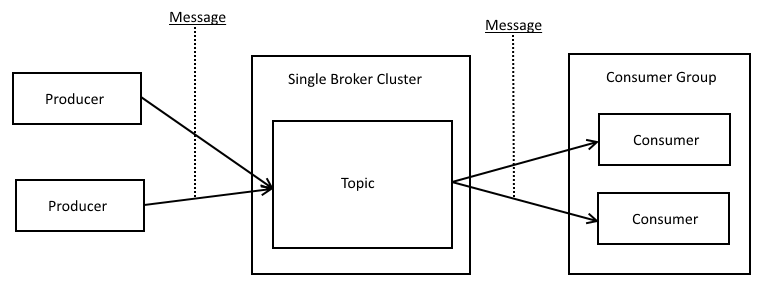
\includegraphics[width=1.0\textwidth]{bilder/kafkaDesign.png}
\caption{Apache Kafka Architektur - Single Broker Cluster
\label{fig:kafkaDesign}}
\end{figure}

Abbildung \ref{fig:kafkaDesign} zeigt ein Beispiel mit einem \textit{Single Broker Cluster} als Server. Das Kafka-Cluster kann auch aus mehreren \textit{Brokern} bestehen. Die Installationsanleitung in Anhang \ref{section:kafkainstall} zeigt eine Konfiguration für ein \textit{Single Broker Cluster}. Für ein \textit{Multi Broker Cluster} werden separate Konfigurationen der Kafka-Maschinen und ein Apache Zookeeper-Cluster benötigt. In der Abbildung \ref{fig:kafkaDesign} werden Nachrichten an das \textit{Topic} von Zwei \textit{Producern} gesendet. Aus der \textit{Consumer Group} holen Zwei \textit{Consumer} Nachrichten aus dem \textit{Topic} ab. Für die Koordination der Nachrichten greifen der \textit{Server}, die \textit{Producer} und die \textit{Consumer} im Hintergrund auf Apache Zookeeper zu. Für die horizontale Skalierung kann ein Apache Zookeeper Cluster genutzt werden. In einem Kafka-Cluster können maximal 255 Knoten existieren. Pro Konfiguration muss jeder Knoten eine eigene Identität unter der \textit{Broker-Id} festgelegt bekommen. Mehrere Knoten mit gleicher Identität führen zu einem unvorhersagbaren \textit{Cluster}-Verhalten. \citelit[S. 28]{garg2013apache}

Sobald Nachrichten von \textit{Consumern} in einem Kafka-Cluster empfangen werden, werden diese lokal innerhalb einer Apache Zookeeper-Maschine im Dateisystem gespeichert. In einem \textit{Consumer} werden die Nachrichten mit einem iterativen Zähler im \textit{Offset} gespeichert. Durch die Angabe des \textit{Offset} ist es möglich Nachrichten von einer \textit{Topic}-Partition ab einer bestimmten \textit{Offset}-Position abzuholen. Beim Speichern der Nachrichten nutzt Apache Kafka die \textit{zero-copy}-Optimierung \citelit{ibmZeroCopy}. Dabei wird die Nachricht in den Linux Page Cache einmalig geschrieben. Weitere Abfragen der Nachrichten werden vom Page Cache geliefert. Durch die zero-copy-Optimierung werden 4 context-switches pro Abfrage in einem Prozess reduziert. \citeint[Kap. 4.3]{kafka:documentation}

In Kafka wird die Reihenfolge von Nachrichten, die von einer \textit{Topic}-Partition abgeholt wird, garantiert. Die Reihenfolge von unterschiedlichen Partitionen kann allerdings abweichen und wird nicht garantiert. In Apache Kafka können Nachrichten mit der \textit{Gzip\footnote{Kompressionswerkzeug: gzip -- \url{http://www.gzip.org/}}}-Anwendung oder der \textit{Snappy\footnote{Kompressionsbibliothek: snappy -- \url{https://code.google.com/p/snappy/}}}-Bibliothek komprimiert werden. Nachrichten werden von Kafka nach einer Verarbeitung in einem \textit{Consumer} abschließend nicht gelöscht. Durch das einstellbare \gls{glo:sla} ist es möglich Nachrichten erst nach einer definierten Zeitspanne zu löschen. In einem \textit{Consumer}-Ausfall ist es durch diese Technik möglich, Nachrichten mit einem neuen bzw. bestehenden \textit{Consumer} erneut abzufragen, also Nachrichten neu einzuspielen. Dennoch sind bei der Übernahme Nachrichten-Duplikate möglich. Eine Anwendung die Kafka einsetzt und mit Duplikaten umgehen muss, muss eine Logik zur Erkennung von Duplikaten bereitstellen.
So wird beim Einsatz von mehreren \textit{Consumern} die Datenkapazität vervielfacht. Nachrichten sind verloren, falls ein \textit{Broker} mit nicht abgeholten Nachrichten ausfällt. \citelit[S. 4, Kap. 3.3]{apache:kafka:kreps2011kafka}

Aus dem Apache Kafka Archiv \citeint{kafka:GitHubApacheMirror} wurde ein Beispiel für die Verwendung von \textit{Producer} und \textit{Consumer} im Anhang unter dem Quelltext \ref{lst:kafkaProducer} und \ref{lst:kafkaConsumer} abgelegt. Beide Klassen erben von der Java \textit{Thread}-Klasse. In einer externen Klasse können beide erweiterten \textit{Threads} instanziiert und mit der \textit{start}-Methode ausgeführt werden. Im \textit{Producer}-Quelltext wird innerhalb der \textit{run}-Methode in einer Schleife eine Nachricht dauerhaft an einen übergebenen \textit{Topic} gesendet. Im \textit{Consumer}-Quelltext wird ebenfalls in der \textit{run}-Methode über ein \textit{Mapping} der \textit{KafkaStream} für das übergebene \textit{Topic} geholt und über den \textit{ConsumerIterator}, solange Nachrichten eintreffen, die Nachrichten in der Konsole ausgegeben. In beiden Implementierungen wird zuvor eine Konfiguration für das Kafka-Cluster gesetzt. Im Quelltext \ref{lst:kafkaProducer} und \ref{lst:kafkaConsumer} liegt eine hierarchische Benennung vor. Die Klasse KafkaStream liegt z.B. im Namensraum "`kafka.consumer.KafkaStream"'. Die Hierarchie wird durch den Punkt abgetrennt. Spezifiert wird von links nach rechts. Beim Synchronisieren zwischen Producer und Consumer werden über Apache Zookeeper Watcher Listener Konfigurationen aktualisiert.

\begin{table}[ht!]
	\centering
		\begin{tabular}{@{}ll@{}} \toprule
			\textbf{Kriterium} & \textbf{Bewertung} \\ \midrule
			Architektur & Strukturierte Peer-to-Peer-Architektur \\
			Prozesse und Threads & Client-Server Cluster, Consumer Pull-Modell \\
			Kommunikation & TCP-basiert mit Apache Zookeeper \\
			Namenssystem & Hierarchische Benennung \\
			Synchronisierung & Apache Zookeeper Watcher \\
			Pipelining und Materialisierung & Publishing als Consumer \\
			Konsistenz und Replikation & Replikation \\
			Fehlertoleranz & Fail-Fast Strategie unter Supervision \\ %CRC removal of bad CRCs -> self healing?
			Sicherheit & Nur eigene Maßnahmen \\
			Erweiterung & Eigenentwicklung und Community-Beiträge \\
			Qualität & At-least-once delivery, time-based \gls{glo:sla} 7 Tage \\
			\bottomrule			
		\end{tabular}
	\caption{Bewertung Apache Kafka}
	\label{tab:bewkafka}
\end{table}

Apache Kafka kann \textit{Topic}-Partitionen replizieren. Mit einem \textit{Replication}-Faktor kann die Anzahl der Replikate in der Konfiguration für einen \textit{Topic} eingestellt werden. Das erste registrierte \gls{glo:isr} bekommt die führende Rolle. Weitere Replikate übernehmen den Status des \textit{Follower}, dem Folgenden. Falls der führende \gls{glo:isr} abstürzt, wird durch den Algorithmus \textit{PacificA} \citelit{pacifica} aus den \textit{Followern} der nächste führende \gls{glo:isr} bestimmt. \citeint[Kap. 4.7]{kafka:documentation}

Da Apache Kafka auf einem Publish-Subscribe-Verfahren aufbaut ist die Wiederbenutzung bzw. Weitergabe von Nachrichten nur unter Angabe eines weiteren \textit{Topic} möglich. Dafür sind mindestens ein weiterer \textit{Publisher} und \textit{Consumer} zu implementieren. Aggregatoren und Operatoren, sowie es unter dem Referenzmodell Aurora/Borealis angeboten wird, kann unter Apache Kafka in der Hochsprache Scala oder Java in einem Producer entwickelt werden. Auch in der Sicherheit fehlen noch Anforderungen zur Authentifizierung und Verschlüsselung innerhalb des Kafka-Clusters \citeint{kafka:security}. Erweiterungen für das Monitoring werden über \gls{glo:jmx} angeboten. Eine Integration in ein Monitoringsystem wie Nagios kann mit dem Java JMX Nagios Plugin\footnote{Java JMX Nagios Plugin: check\_jmx -- \url{http://exchange.nagios.org/directory/Plugins/Java-Applications-and-Servers/check\_jmx/details}} erfolgen.

In diesem Kapitel wurde die Installation und ein Beispielanwendung für den Austausch von Nachrichten gezeigt. Auf spezielle Eigenschaften wie das zero-copy \citelit{ibmZeroCopy}, Parallelisierung und Replikation wurde eingegangen. Außerdem wurden die Bewertungskriterien aus Tabelle \ref{tab:bewkafka} für Apache Kafka erläutert. Im nächsten Kapitel wird nun Apache Flume vorgestellt.


% jkreps / benchmark-commands.txt: https://gist.github.com/jkreps/c7ddb4041ef62a900e6c

\section{Apache Flume}

Nachdem Apache Storm und Apache Kafka bewertet wurden, wird als nächstes Apache Flume vorgestellt. Apache Flume wurde ursprünglich von Jonathan Hsieh im Jahr 2009 und der Firma Cloudera entwickelt und wird als ein verteiltes, zuverlässiges und verfügbares System für effizientes Sammeln, Aggregieren und Bewegen großer Datenmengen von Protokolldaten von verschiedene Quellen zu einem Zentralen Datenspeicher beschrieben \citeint{flume:Proposal}. Am 29 Juni 2010 wurde Apache Flume unter der Apache License Version 2.0 veröffentlicht und am 20 Juni 2012 in die Apache Software Foundation überführt \citeint{flume:IncubationStatus}. Nachdem Apache Flume am 13 Juni 2013 in den Apache Incubations Prozess überführt wurde, wurde nach Version 0.9.5 in der neuen Fassung ab Version 1.0.0-incubating eine weitreichende Refaktorierung\footnote{Refaktorierung ist ein Prozess in der Software-Entwicklung, um die interne Struktur zu verbessern, während das äußere Verhalten unverändert bleibt \citelit[S. 9]{Fowler99}.} von Arvind Prabhakar, Prasad Mujumdar und Eric Sammer mit der Unterstützung von Jonathan Hsieh, Patrick Hunt und Henry Robinson durchgeführt \citeint{flume:flumeNg}. Die Abkürzung \gls{glo:ng} in der neuen Version von Apache Flume steht für die Weiterentwicklung und der Refaktorierung \citeint{flume:flumeNgRefactoring}. In dieser Arbeit wird ausschließlich die neue Fassung der Apache Foundation ab Version 1.0.0-incubating vorgestellt. In der Tabelle \ref{tab:vorflume} wird eine Kurzübersicht über Apache Flume gezeigt. Dabei wird unter den Hauptentwicklern die ersten drei Entwickler der neuen Fassung Flume-NG und abschließend die drei Entwickler aus der ursprünglichen Fassung aufgelistet.

Apache Flume wurde aus der Anforderung heraus als ein allgemeines Werkzeug Daten für einen Datenlieferanten für Apache Hadoop\footnote{Apache Hadoop ist eine Bibliothek von Anwendungen für das verteilte Rechnen von großen Datenmengen in einem Cluster. Es besteht aus dem Dateisystem \gls{glo:hdfs}, dem Algorithmus MapReduce und dem Aufgabenplaner Yarn. \citeint{hadoop:home}} entwickelt. In der Entwicklung von der Apache Flume wird gleichzeitig eine Anbindung an das Apache Hadoop Dateisystem \gls{glo:hdfs} als \textit{HDFS Sink} bereitgestellt. Dennoch sind weitere Sink-Implementierungen gegeben und möglich. In dieser Arbeit steht der Fokus in der kontinuierlichen Datenverarbeitung, weshalb die Schnittstelle zu Apache Hadoop nicht näher beleuchtet wird. \citelit[S. 1]{flumeDistributed}

\begin{table}[tbp]
	\centering
		\begin{tabular}{@{}ll@{}} \toprule
			\textbf{Faktum} & \textbf{Beschreibung} \\ \midrule
			Hauptentwickler & Arvind Prabhakar, Prasad Mujumdar, Eric Sammer \\
			& Jonathan Hsieh, Patrick Hunt, Henry Robinson \\
			Stabile Version & 1.5.0.1 vom 16.06.2014 \\ 
			Entwicklungsstatus &  Aktiv \\
			Entwicklungsversion & 1.6.0 \\
			Sprache & Java \\
			Betriebssystem & Linux/Unix konform, kein Support für Windows  \\
			Lizenz & Apache License version 2.0 \\
			Webseite & \citeint{flume:home} \\
			Quelltext & \citeint{flume:GitHubApacheMirror} \\			
			\bottomrule			
		\end{tabular}
	\caption{Kurzübersicht Apache Flume}
	\label{tab:vorflume}
\end{table}


Die Architektur von Apache Flume besteht aus mehreren einzelnen Maschinen die als \textit{Agents} bezeichnet werden. Jedem \textit{Agent} wird über eine Konfigurationsdatei die Verbindung zu einem anderen \textit{Agent} angegeben. Ein \textit{Agent} besteht immer aus einer Quelle \textit{Source}, einem Kanal \textit{Channel} und einer Ausgabe \textit{Sink}. Zwischen der \textit{Source}, dem \textit{Channel} und dem \textit{Sink} werden Nachrichten die \textit{Flume events} ausgetauscht. Daten werden von der \textit{Source} in \textit{Flume events} umgewandelt und an einen oder mehrere \textit{Channels} geschrieben. Ein \textit{Channel} ist der Bereich in dem \textit{Events} gehalten und weiter an die den \textit{Sink} gereicht werden. Der \textit{Sink} erhält ausschließlich Events von einem \textit{Channel}. In einem Agent kann es mehrere \textit{Sources}, \textit{Channels} und \textit{Sinks} geben.

\begin{table}[ht!]
	\centering
		\begin{tabular}{@{}ll@{}} \toprule
			\textbf{Kriterium} & \textbf{Bewertung} \\ \midrule
			Architektur & Strukturierte Peer-to-Peer-Architektur \\
			Prozesse und Threads & Client-Server-Modell und \gls{glo:rpc} \\
			Kommunikation & Streamorientierter synchroner Übertragungsmodus \\
			Namenssystem & Hierarchische Benennung \\
			Synchronisierung & Dezentraler Algorithmus \\
			Pipelining und Materialisierung & Agent chaining \\
			Konsistenz und Replikation & Replikation und Multiplexing \\
			Fehlertoleranz & Load balancing und Failover \\ 
			Sicherheit & FileChannel Verschlüsselung, \\
			& vereinzelte \acrshort{glo:sasl}-Sink-Integration \\
			Erweiterung & Eigenentwicklung und Community-Beiträge \\
			Qualität & FileChannel \gls{glo:wal} \\
			\bottomrule			
		\end{tabular}
	\caption{Bewertung Apache Flume}
	\label{tab:bewflume}
\end{table}

%Instead of focusing on analytics, Flume focuses primarily upon data transport and integration with a wide set of data sources and data destinations.
%http://www.ibm.com/developerworks/opensource/library/bd-flumews/index.html
%http://blog.cloudera.com/blog/2013/01/how-to-do-apache-flume-performance-tuning-part-1/
%\citelit{rfc4422}

\section{Apache S4}


Nach der Vorstellung von Apache Storm, Kafka und Flume wird in diesem Kapitel Apache S4 vorgestellt. Apache S4 ist eine Abkürzung und steht für Simple Scalable Streaming System und wird von Flavio Junqueira als allgemeine, verteilte, skalierbare, teilweise fehlertolerante und steckbare Plattform bezeichnet \citeint{s4:Proposal}. Zunächst soll eine Kurzübersicht einen ersten Einblick in Apache S4 geben. Anschließend werden die Bewertungskriterien erläutert und vorgestellt.

Die Architektur von Apache S4 baut auf einem Apache Zookeeper Cluster auf und besteht aus mehreren Apache S4 \textit{Cluster}, \textit{Processing Nodes}, \textit{Apps}, \textit{Processing Elements} und dem \textit{Communication Layer}. \textit{Apps} sind Java Archive, die in einem Apache S4 \textit{Cluster} bereitgestellt werden. Die Größe eines \textit{Clusters} entspricht der Anzahl der \textit{Tasks}. Pro \textit{Task} muss jeweils eine \textit{Processing Node} als selbständiger Prozess gestartet werden. Eine \textit{Procssing Node} dient als Container für mehrere \textit{Processing Elements}. \textit{Apps} bestehen aus einem Graphen von \textit{Processing Elements} und \textit{Streams}. Ein \textit{Processing Element} kommuniziert asynchron über unterschiedliche \textit{Cluster} per \textit{Streams}. Der Nachrichtenaustausch erfolgt über den \textit{Communication Layer}. 

\begin{table}[tbp]
	\centering
		\begin{tabular}{@{}ll@{}} \toprule
			\textbf{Faktum} & \textbf{Beschreibung} \\ \midrule
			Hauptentwickler & Matthieu Morel, Kishore Gopalakrishna, Flavio Junqueira \\
			& Leo Neumeyer, Bruce Robbins, Daniel Gomez Ferro \\
			Stabile Version & 0.6.0 vom 03.06.2013 \\ 
			Entwicklungsstatus &  Moderat \\
			Entwicklungsversion & 0.7.0 \\
			Sprache & Java \\
			Betriebssystem & plattformunabhängig, benötigt die Java Virtual Machine \\
			& und Apache Zookeeper \\
			Lizenz & Apache License version 2.0 \\
			Webseite & \citeint{s4:home} \\
			Quelltext & \citeint{s4:GitHubApacheMirror} \\			
			\bottomrule			
		\end{tabular}
	\caption{Kurzübersicht Apache S4}
	\label{tab:vors4}
\end{table}

Abbildung \ref{fig:s4ProcessingNode} zeigt Zwei Processing Nodes mit mehreren Processing Elements. Ein Raw Event wird von der äußeren Umgebung an die erste Processing Node in den Event Listener übergeben. Der Dispatcher erhält die verarbeitete Nachricht von einem Processing Element und leitet diese an den Emitter weiter. Der Emitter setzt die Nachricht in einen Stream. Der Stream wird vom Communication Layer an die zweite Processing Node vermittelt. Die Verarbeitung wird von der zweiten Processing Node durchgeführt. Das User Interface Model holt sich die Nachrichten vom neuen Stream ab und stellt die Information in der Benutzerschnittstelle dar.

Eine spezielle Implementierung einer Nachricht muss von der Klasse \textit{Event} erben, aus einem Schlüssel/Wert-Tupel bestehen und an einen \textit{Stream} weitergegeben werden können. Mit der Erweiterung der Basisklasse \textit{AdapterApp} kann ein \textit{Stream} erzeugt werden. Ein Beispiel wird im Anhang \ref{lst:s4HelloInputAdapter} gezeigt. Dabei wird auf eine Netzwerkverbindung mit dem Anschluss 15000 gehört. Bei erfolgreicher Verbindung wird der Inhalt gelesen und in einen \textit{Stream} gesetzt. 

\begin{figure}[htb!]
\centering
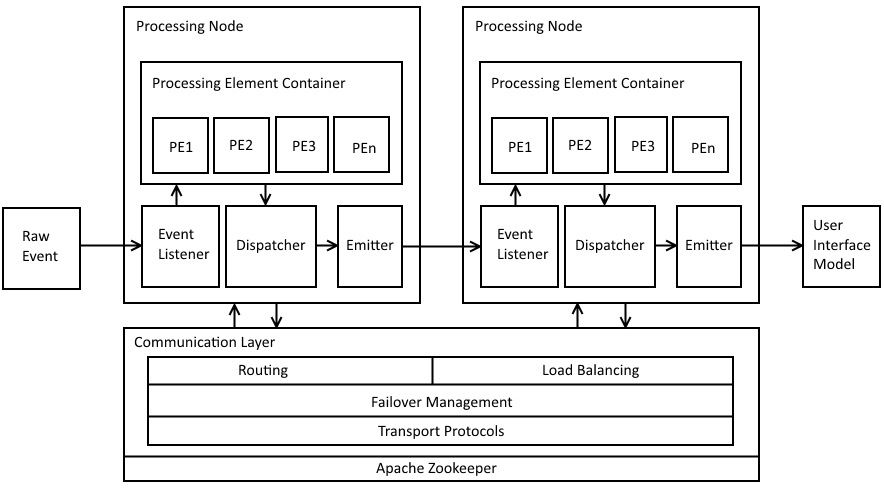
\includegraphics[width=1.0\textwidth]{bilder/s4ProcessingNodes.png}
\caption{Apache S4 Processing Nodes
\label{fig:s4ProcessingNode}}
\end{figure}

In einem \textit{Processing Element} wird die Datenverarbeitung durchgeführt. In Apache S4 gibt es nur zwei Typen von \textit{Processing Elements}, ein Schlüssel-loses und ein Schlüssel-behaftetes \textit{Processing Element}. Der Schlüssel-lose Typ kann unterschiedliche Apache S4 Nachrichten empfangen. Der Schlüssel-behaftete Typ kann nur Apache S4 Nachrichten mit einem definierten Schlüssel in der Nachricht empfangen. Spezielle Aggregate und Operatoren von Nachrichten müssen in \textit{Processing Elements}-Klassen explizit implementiert werden. Ein \textit{Processing Element} besteht aus Zwei Teilen, dem \textit{Prototype} und der \textit{Instance}. Der \textit{Prototype} erbt von der Basisklasse \textit{ProcessingElement} und behandelt eingehende Nachrichten. Die \textit{Instance} erbt von der Basisklasse \textit{App} und behandelt den Anwendungsstart und Anwendungsstop. Im Anhang \ref{lst:s4HelloAppProcessingElementInstance} wird ein Beispiel für das Erzeugen eines \textit{Streams} "`names"' und die Weitergabe der Nachrichten an einen \textit{Stream} gezeigt. \citeint{s4:overview}

\begin{figure}[htb!]
\centering
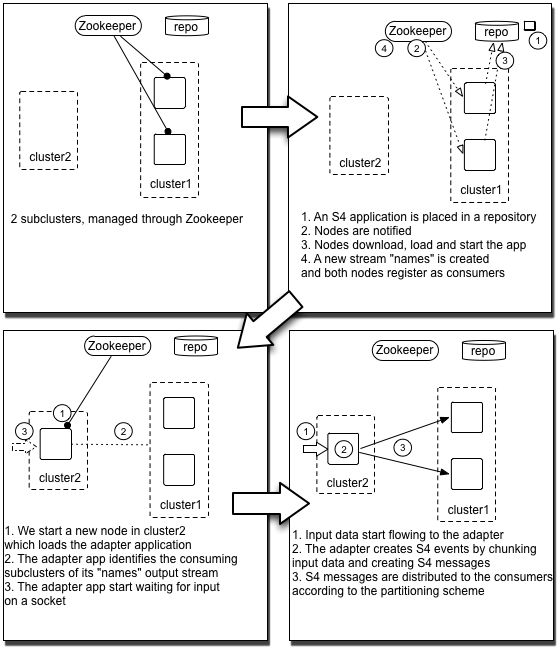
\includegraphics[width=1.0\textwidth]{bilder/s4SampleAppDeployment.png}
\caption{Apache S4 HelloApp Beispiel
\label{fig:s4HelloApp}}
\end{figure}

In Abbildung \ref{fig:s4HelloApp} wird das Beispiel \ref{s4:beispielHelloApp} aus der Apache S4 Installation im Anhang \ref{sec:s4install} gezeigt. Die Abbildung \ref{fig:s4HelloApp} wurde aus der Dokumentation \citeint{s4:walkthrough} entnommen. Zuerst werden Zwei Cluster \textit{cluster1} und \textit{cluster2} in einem Apache Zookeeper \textit{Cluster} bereitgestellt. Anschließend wird im \textit{Repository} die S4 Anwendung \textit{myApp} hinzugefügt. Die Apache S4 \textit{Nodes} werden über Apache Zookeeper informiert und die Anwendung wird gestartet. Ein neuer \textit{Stream} "`names"' wird erstellt und beide \textit{Nodes} werden als \textit{Consumer} registriert. Anschließend wird im \textit{Cluster} \textit{cluster2} die \textit{HelloInputAdapter}-Anwendung gestartet. Beim Bereitstellen der Anwendung im \textit{Cluster} \textit{cluster2} wird der \textit{Stream} "'names"' als Identität für den Ausgabestrom gesetzt. Die \textit{HelloInputAdapter}-Anwendung ist nach dem Starten aktiv und wartet auf Dateneingang. Abschließend werden eintreffende Daten vom \textit{Cluster} \textit{cluster2} in Apache S4-Nachrichten umgewandelt und zur weiteren Datenbehandlung an die \textit{Consumer} verteilt.


Nachrichten werden in Apache S4 zwischen den \textit{Nodes} durch den \textit{Communication Layer} übertragen. Der \textit{Communication Layer} nutzt für die Koordination der Nachrichten zwischen den Apache S4 \textit{Nodes} Apache Zookeeper. Um Nachrichten an die \textit{Nodes} im Apache S4 \textit{Cluster} zu senden, können spezielle Bindungen in verschiedenen Programmiersprachen implementiert werden. Durch ein steckbares Design können unterschiedliche Nachrichtenprotokolle wie zum Beispiel Apache Avro oder Apache Thrift eingesetzt werden. Eine Implementierung für das \gls{glo:udp} \citeint{s4:classUdpEmitter} und dem \gls{glo:tcp} \citeint{s4:classTcpEmitter} wird von Apache S4 bereits unterstützt. \citelit[S. 4, Kap. II D]{s4:Neumeyer}

Die Fehlertoleranz in Apache S4 wird durch die \textit{Fail-Fast} Strategie von Apache Zookeeper übernommen. In einem Apache S4 Cluster mit Zwei \textit{Tasks} und Vier gestarteten \textit{Nodes}, sind Zwei \textit{Nodes} Aktiv und Zwei \textit{Nodes} im \textit{Standby}-Betrieb. Wenn Apache Zookeeper einen \textit{Session-Timeout} einer aktiven \textit{Node} feststellt, wird sofort eine \textit{Standby-Node} aktiviert. Die anderen \textit{Nodes} werden durch den \textit{Communication Layer} über neue aktive \textit{Node} informiert und neue Nachrichten werden umgeleitet. Apache S4 \textit{Nodes} nutzen für die Datenverarbeitung den lokalen Speicher von Apache Zookeeper. Im Fehlerfall geht der Zwischenspeicher einer Apache Zookeeper \textit{Node} verloren. Damit die Daten nicht verloren gehen, kann mit dem \textit{Checkpointing}-Mechanismus über die Konfiguration eine Datensicherung in einem externen Datenlager erfolgen. Beim Start der neuen \textit{Nodes} aus dem \textit{Standby}-Betrieb kann die Datensicherung in den lokalen Speicher zurückgeschrieben werden. In \citelit{valles2012analysis} untersucht Vall{\'e}s verschiedene Ansätze von \textit{Checkpointing} und zeigt eine geringe Performanz der Standardimplementierung gegenüber einer Implementierung mit Apache HBase\footnote{Apache HBase ist eine Apache Hadoop Datenbank, ein verteilter, skalierbarer Big Data-Speicher \citeint{hbase:home}.}. \citeint{s4:faultTolerance}

\begin{table}[!ht]
	\centering
		\begin{tabular}{@{}ll@{}} \toprule
			\textbf{Kriterium} & \textbf{Bewertung} \\ \midrule
			Architektur & Strukturierte Peer-to-Peer-Architektur \\
			Prozesse und Threads & Client-Server-Modell \\
			Kommunikation & TCP-basiert und UDP-basiert via Apache Zookeeper \\
			Namenssystem & Hierarchische Benennung \\
			Synchronisierung & Communication Layer \\
			Pipelining und Materialisierung & Chaining von Processing Elements  \\
			Konsistenz und Replikation & Consistent hashing, Checkpointing \\
			Fehlertoleranz & Failover und Checkpointing \\ 
			Sicherheit & Nur eigene Maßnahmen \\
			& Monitoring mit JMX pro Node \\
			Erweiterung & Modulare Eigenentwicklung \\
			Qualität & Nur eigene Entwicklung für \gls{glo:qos}  \\
			\bottomrule			
		\end{tabular}
	\caption{Bewertung Apache S4}
	\label{tab:bews4}
\end{table}

Bei der Sicherheit sind eigene Maßnahmen notwendig. Nachrichten werden im Klartext oder binär übertragen. Die Verbindung zwischen den einzelnen \textit{Processing Nodes} findet unautorisiert statt. Für die Autorisierung und Verschlüsselung ist eine spezielle Implementierung des \textit{Communication Layer} und der einzelnen \textit{Processing Elements} notwendig. Weiterhin ist eine Verschlüsselung des lokalen Speichers von Apache Zookeeper in einem offenen Netz zu empfehlen. Über \gls{glo:jmx} können Metriken eines Apache S4 Clusters abgefragt werden \citeint{s4:metrics}. \gls{glo:qos} wird in \citelit[S. 3, Kap. II B]{s4:Neumeyer} als anwendungsspezifisch eingestuft. In einer spezifischen Anwendung muss daher eine eigene Implementierung für das \gls{glo:qos} in Apache S4, innerhalb von \textit{Processing Elements} erfolgen.


Diese Kapitel stellt das Streaming Framework Apache S4 vor. Es wurde die Installation von Apache S4 beschrieben und im Anhang \ref{sec:s4install} eine Anleitung abgelegt. Weiterhin erfolgte eine Erklärung der Architektur und der Informationsfluss in einem Apache S4 \textit{Cluster} wurde erläutert. Es wurde die Fehlertoleranz in Zusammenhang von Apache Zookeeper und die Replikation mit \textit{Checkpointing} beschrieben und zuletzt auf eine geringe Sicherheit, Monitoring und Qualität hingewiesen. Nach der Vorstellung der Streaming Frameworks werden im folgenden Kapitel die wesentlichen Kernelemente der einzelnen Streaming Frameworks zusammengefasst.

\section{Zusammenfassung}

\chapter{Anwendungsfall und Prototyp}

\chapter{Auswertung}
\section{Benchmark Ergebnisse}
\section{Erkenntnis}

\chapter{Schlussbetrachtung}
\section{Zusammenfassung}
\section{Einschränkungen}
\section{Ausblick}



%%%%%%%%%%%%%%%%%%%%%%%%%%%%%%%%%%%%%%%%%%%%%%%%%%%%%%%%%%%%%%%
%% Verzeichnisse

\chapter{Verzeichnisse}
%\addcontentsline{toc}{chapter}{Verzeichnisse}

\bibliographystylelit{geralpha}
\bibliographylit{literaturVerzeichnis}
\addcontentsline{toc}{section}{Literaturverzeichnis}

%\newpage
\bibliographystyleint{geralpha}
\bibliographyint{internetQuellen}
\addcontentsline{toc}{section}{Internetquellen}

%\newpage
\listoffigures
\addcontentsline{toc}{section}{Abbildungsverzeichnis}
\clearpage
\cleardoublepage
%\newpage
\listoftables
\addcontentsline{toc}{section}{Tabellenverzeichnis}
\clearpage
\cleardoublepage
\lstlistoflistings 
\addcontentsline{toc}{section}{Quellenverzeichnis}
\clearpage
\cleardoublepage

%%%%%%%%%%%%%%%%%%%%%%%%%%%%%%%%%%%%%%%%%%%%%%%%%%%%%%%%%%%%%%%
%% Anhang

\clearpage\newpage
\begin{appendix}
  %%
%% Beuth Hochschule für Technik --  Abschlussarbeit
%%
%% Anhang
%%
%%%%%%%%%%%%%%%%%%%%%%%%%%%%%%%%%%%%%%%%%%%%%%%%%%%%%%%%%%%%%%%%%%%%%

\chapter{Zusätze}

\setglossarysection{section}
\printglossary[type=\acronymtype,title=Abkürzungen]


\section{Quelltext}
\label{section:quelltext}

\lstinputlisting[language=XML, label=lst:aurorborealisdeoployconf, caption=Aurora Borealis Konfiguration für die Verteilung]{anhangQuelltext/borealismytestdist-deploy.xml}

\lstinputlisting[language=XML, label=lst:aurorborealisqueryconf, caption=Aurora Borealis Konfiguration für die Abfragen]{anhangQuelltext/borealismytestdist.xml}

\lstinputlisting[language=C++, label=lst:aurorborealismytest, caption=Aurora Borealis Testanwendung]{anhangQuelltext/mytestdist.cc}

\lstinputlisting[language=JAVA, label=lst:WordCountTopology, caption=Apache Storm WordCount Demo]{anhangQuelltext/WordCountTopology.java}

\lstinputlisting[language=JAVA, label=lst:kafkaProducer, caption=Apache Kafka Producer Beispiel]{anhangQuelltext/kafkaProducer.java}

\lstinputlisting[language=JAVA, label=lst:kafkaConsumer, caption=Apache Kafka Consumer Beispiel]{anhangQuelltext/kafkaConsumer.java}


\section{Installationsanleitung Aurora/Borealis}
\label{sec:aurborinstall}


In dieser Anleitung wird die Installation von Aurora Borealis in kleinen Unterkapiteln vorgestellt. Diese Anleitung setzt ein Vorwissen in der Verwendung und Administration von Linux voraus. Zudem wird Erfahrung von Erzeugen von Anwendungen aus Quelltext benötigt. Zum Beispiel können Konflikte auftreten, wenn neue Versionen von Bibliotheken benötigt werden. Dabei müssen die Abhängigkeiten beachtet und abhängige Konflikte aufgelöst werden. Bevor das Erstellen der Anwendung beginnt werden zuerst die Voraussetzungen bestimmt und erläutert. Anschließend wird mit Quelltextfragementen und Kommandozeilenausschnitten schrittweise die Eingabe und Ausgabe gezeigt.


\subsection{Voraussetzungen am Betriebssystem}

Die Installation von Aurora Borealis benötigt ein auf linuxbasiertes Betriebsystem. Auf dem Betriebssystem Microsoft Windows wurde eine Erstellung des Quelltextes von Aurora Borealis bisher nicht durchgeführt. Zum Zeitpunkt der Erstellung dieser Anleitung wird versucht ein Ist-Zustand der Anwendung aufzunehmen. Für das Verteilte System Aurora Borealis wird die Linuxdistribution Debian benutzt.


\subsection{Voraussetzung Erstellsystem}

Einige Pakete bzw. Bibliotheken werden für das Erstellen von Aurora Borealis benötigt. Als Paketverwaltung wird unter Debian \textit{apt} benutzt. Mit dem Befehl \textit{apt-get} können Pakete dem Betriebssystem aus dem Standard Debian Paket-Repository hinzugefügt werden. Folgende Liste zeigt benötigte Pakete für das Erstellen von Aurora Borealis:

\begin{itemize}
	\item build-essentials (gcc, g++, configure, make)
	\item ccache
	\item antlr
	\item libxerces-c3.1 (Xerces-c: Used by Borealis to parse XML)
	\item libtool
	\item autoconf
	\item automake
	\item libdb5.1 (Berkeley-Db)
	\item glpk (GNU Linear Programming Kit)
	\item gsl (GNU Scientific Library - collection of routines for numerical analysis: used for predictive queries)
	\item opencv (open source computer vision: used for array processing)
	\item doxygen (serves to generate documentation)
	\item openjdk-7-jdk (java 7)
\end{itemize}

Da die letzte Version von Aurora Borealis aus dem Jahr 2008 ist, gibt es beim Erstellen mit neueren Versionen von \textit{gcc} und \textit{g++} Fehler. 
Damit die neue Version von \textit{gcc} benutzt werden kann muss der Quelltext der Version aus 2008 angepasst werden. Eine erste Anpassung wurde versucht durchzuführen. Zum Beispiel sind bestimmte Standardmethoden direkt angegeben worden. Trotzdem wurden weiterführende Fehler gefunden. Als Fehler wird \textit{missing \#include} gemeldet. Im \textit{borealis} Verzeichnis sind 239 \textit{Makefiles} vorhanden. Alle \textit{Makefiles} und die darin verbundenen Quelltext-Dateien müssen auf die neue Version geprüft werden. Eine Stabile Version mit den neuen Anpassungen kann nur durch effektive Testläufe gewährleistet werden. Um den Quelltext von Aurora Borealis nicht anzupassen kommt die ältere Version 4.0 von Debian zum Einsatz. In diesem Fall muss die Liste von benötigten Paketen angepasst werden:

\begin{itemize}
	\item build-essentials (gcc, g++, configure, make)
	\item ccache
	\item antlr
	\item libxerces27 (Xerces-c: Used by Borealis to parse XML)
	\item libtool
	\item autoconf
	\item automake
	\item libdb (Berkeley-Db)
	\item glpk (GNU Linear Programming Kit)
	\item gsl (GNU Scientific Library - collection of routines for numerical analysis: used for predictive queries)
	\item opencv (open source computer vision: used for array processing)
	\item doxygen (serves to generate documentation)
	\item sun-java5-jdk (Java 1.5 von SUN)
	\item libexpat1-dev
	\item ibreadline5-dev
\end{itemize}


\subsection{Quelltext von Aurora Borealis herunterladen}

Die Datei liegt nicht in einer öffentlichen Versionsverwaltung, sondern kann als Archive von der Brown University unter folgendem Link heruntergeladen werden:
\url{http://www.cs.brown.edu/research/borealis/public/download/borealis_summer_2008.tar.gz} \\
Alternativ liegt der Quelltext und das Installationsmedium Debian 4.0 als \gls{glo:iso} 9660 Abbild im Ordner \textit{anhangSoftwareZusatz}. Nachdem die Anwendung im Verzeichnis \textit{/opt} liegt kann sie im gleichen Verzeichnis entpackt werden. Im Verzeichnis liegen anschließend zwei Unterordner \textit{borealis} und \textit{nmstl}.


\subsection{Kommandozeile Umgebungsvariablen festlegen}

Unter Debian wird für die Kommandozeile die Shell \textit{Bash} eingesetzt. Wenn eine Shell eröffnet wird, wird die Datei \textit{.bashrc} im Benutzerverzeichnis aufgerufen. Darin werden Benutzerabhängige Konfigurationen abgelegt. Die Umgebungsvariablen für Aurora Borealis werden im folgenden Abschnitt gezeigt:
\begin{verbatim}
alias debug='export LOG_LEVEL=2'
alias debug0='export LOG_LEVEL=0'
export PATH=${PATH}:/opt/nmstl/bin:/${HOME}/bin
export CLASSPATH='.:/usr/share/java/antlr.jar:$CLASSPATH'
export JAVA_HOME=$(readlink -f /usr/bin/javac | sed "s:/bin/javac::")
export PATH=${JAVA_HOME}/bin:${PATH}
export CXX='ccache g++'
export CVS_SANDBOX='/opt'
export INSTALL_BDB='/usr'
export INSTALL_GLPK='/usr'
export INSTALL_GSL='/usr'
export INSTALL_ANTLR='/usr'
export INSTALL_XERCESC='/usr'
export INSTALL_NMSTL='/usr/local'
export LD_LIBRARY_PATH='/usr/lib'
export ANTLR_JAR_FILE='/usr/share/java/antlr.jar'

mkdir -p bin
alias bbb='/opt/borealis/utility/unix/build.borealis.sh'
alias bbbt='/opt/borealis/utility/unix/build.borealis.sh -tool.head
 -tool.marshal'
alias retool='/bin/cp -f ${CVS_SANDBOX}/borealis/tool/head/BigGiantHead
 ${HOME}/bin; /bin/cp -f ${CVS_SANDBOX}/borealis/tool/marshal/marshal
 ${HOME}/bin'
\end{verbatim}


\subsection{Notwendige Quelltext Anpassung}

Beim Erzeugen wird unter anderen Paketen auch \gls{glo:antlr} benutzt. Während der Erstellens findet ein Fehler auf. Bei der Konfiguration für das \textit{Makefile} wurde ein Pfad fest einprogrammiert. Dieser feste Pfad wird nun durch einen Variable in die Umgebungsvariable \textit{ANTLR\_JAR\_FILE} ausgelagert. Dazu muss in der Datei \textit{/opt/borealis/src/configure.ac} der Inhalt an der Stelle ANTLR\_JAR\_FILE= mit \textit{\$ANTLR\_JAR\_FILE} nach dem Gleichzeichen ausgetauscht werden.


\subsection{Erzeugen von NMSTL}

Borealis benutzt eine angepasste Version von \gls{glo:nmstl}. Im Verzeichnis \textit{/opt/nmstl} werden nun folgende Befehle nacheinander ausgeführt:

\begin{verbatim}
autoconf
./configure
make
make install
\end{verbatim}


\subsection{Erzeugen von Borealis}

In das Verzeichnis \textit{/opt/borealis} zurückspringen und folgende Befehle nacheinander ausführen:

\begin{verbatim}
bbb
bbbt
retool
make install
\end{verbatim}


\subsection{Zusätzliche Informationen}
Der Support für Aurora Borealis ist seit 2008 eingestellt. Weitere Informationen stehen unter folgendem Link:
\url{http://cs.brown.edu/research/borealis/public/install/install.borealis.html}

\section{Installationsanleitung Apache Storm}
\label{sec:storminstall}


In diesem Kapitel wird die Installation von Apache Storm in kleinen Unterkapiteln vorgestellt. Die Anleitung setzt ein Wissen in der Verwendung, Administration und Erzeugen von Anwendungen unter dem Betriebssystem Linux voraus. Zuerst werden Voraussetzungen bestimmt und erläutert. Anschließend wird der Start eines Clusters gezeigt. Zuletzt wird eine Beispiel-Anwendung \textit{WordCount} im \textit{local cluster mode} ausgeführt.


\subsection{Voraussetzungen am Betriebssystem}

Als Betriebssystem wird in dieser Anleitung Linux mit der Deistribution Ubuntu 13.10 verwendet. Apple Mac OS X und Microsoft Windows mit einer Cygwin-Umgebung werden in dieser Anleitung nicht betrachtet. Unter Ubuntu wird für die Installation von Paketen das Kommandozeilen-Werkzeug \textit{aptitude }eingesetzt.


\subsection{Paketabhängigkeiten}

Einige Pakete benötigt Apache Storm zur Laufzeit bzw. werden zum Erzeugen gebraucht. Die folgende Liste stellt die notwendigen Pakete dar:

\begin{itemize}
	\item zookeeper
	\item libtool
	\item autoconf
	\item automake
	\item openjdk-7-jdk
	\item zeromq (evt. nicht im Linux Repository)
	\item jzmq (evt. nicht im Linux Repository)
\end{itemize}

Falls die Pakete zu ZeroMQ in den Paketquellen fehlen, müssen beide manuell erzeugt und dem Betriebssystem hinzugefügt werden. Folgende Kommandozeilen zeigen das Herunterladen, Erzeugen und Bereitstellen von ZeroMQ schrittweise:
\begin{verbatim}
wget download.zeromq.org/zeromq-3.2.4.tar.gz
tar xvfz zeromq-3.2.4.tar.gz
./configure
make 
make install
ldconfig
\end{verbatim}

Apache Storm benutzt zur Kommunikation mit ZeroMQ Java-Bindings. Folgende Kommandozeilenaufrufe müssen zur Installation schrittweise ausgeführt werden:
\begin{verbatim}
wget github.com/zeromq/jzmq/archive/master.zip
./autogen.sh
./configure
make
\end{verbatim}


\subsection{Storm Konfiguration}

Apache Storm in das Verzeichnis /opt herunterladen, entpacken und einen Link \textit{storm} erstellen.
\begin{verbatim}
wget http://apache.openmirror.de/incubator/storm/
	apache-storm-0.9.1-incubating/apache-storm-0.9.1-incubating-src.zip
unzip apache-storm-0.9.1-incubating-src.zip
ln -s storm apache-storm-0.9.1-incubating-src.zip
\end{verbatim}

Die Konfigurationsdatei /opt/storm/conf/storm.yaml öffnen und folgenden Eintrag hinzufügen:
\begin{verbatim}
storm.local.dir: "/opt/storm"
\end{verbatim}


\subsection{Cluster starten}

Zookeeper muss bereits im Hintergraund als Dienst laufen, damit das Storm Cluster starten kann.

Mit folgendem Befehl kann der Zookeeper Dienst auf Aktivität gerpüft werden.
\begin{verbatim}
./zkCli.sh -server 127.0.0.1:2181 
\end{verbatim}

Die folgenden Schritte zeigen nacheinander den Start der Storm Komponenten:

\begin{verbatim}
/opt/storm/bin/storm nimbus
/opt/storm/bin/storm supervisor
/opt/storm/bin/storm ui
\end{verbatim}


\subsection{WordCount Demo im local cluster mode}

Mit git wird zuerst die Beispiel Anwendung WordCount in ein lokales Verzeichnis dublizieren:

\begin{verbatim}
git clone git://github.com/apache/incubator-storm.git
\end{verbatim}

Die Anwendung WordCountTopology wird mit Apache Maven im storm cluster bereitgestellt und ausgeführt:

\begin{verbatim}
mvn -f m2-pom.xml compile exec:java -Dexec.classpathScope=compile 
-Dexec.mainClass=storm.starter.WordCountTopology
\end{verbatim}

Da keine Argumente bei der Ausführung übergeben werden, wird als \textit{cluster} der \textit{LocalCluster} benutzt. In der Java Klasse \textit{WordCountTopology} wird in der \textit{main}-Methode entschieden, ob der LocalCluster benutzt wird. Als Ausgabe werden während der Verarbeitung Log Informationen ausgegeben. Eine Erfolgmeldungs wird ausgegeben, falls das Erstellen und Ausführen auf dem Cluster erfolgreich durchgeführt wurde.

\section{Installationsanleitung Apache Kafka}
\label{section:kafkainstall}


Dieses Kapitel beschreibt schrittweise die Installation von Apache Kafka. Die Installation erfordert Kenntnisse in der Installation und Administration von Anwendungen unter dem Betriebssystem Linux. Eine Installation unter dem Betriebssystem Unix, Max OS X und Microsoft Windows wird in dieser Arbeit nicht behandelt. Bevor die Installation beginnen kann, werden zuerst Voraussetzung an das Betriebssystem aufgezählt. Im Kapitel Installation wird der Quelltext kompiliert und ein erster Start von Kafka wird gezeigt. Abschließend wird eine Konfiguration für ein Kafka Single Broker Cluster vorgestellt und Beispiel zwischen einem Producer, dem Nachrichtenerzeuger und einem Consumer, dem Nachrichtenempfänger gezeigt.


\subsection{Voraussetzungen in Linux}

Als Linux Distribution wird Debian 7 verwendet. Da Apache Kafka auf Scala basiert, werden folgende Linux-Pakete benötigt:

\begin{itemize}
	\item zookeeper
	\item scala
	\item openjdk-7-jdk	
\end{itemize}

Das Hinzufügen der Linux-Pakete kann mit der Paketverwaltung \textit{apt-get} oder mit \textit{aptitude} erfolgen. Weitere Paket-Abhängigkeiten werden automatisch vorgeschlagen. Die Installation der Paket-Abhängigkeiten ist zwingend und Konflikte müssen aufgelöst werden.  

Um die notwendige Abhängigkeiten, wie unter Java mit Maven\footnote{Maven: Java Build Werkzeug \url{http://maven.apache.org/}} unter Scala aufzulösen, wird das Werkzeug \gls{glo:sbt} von der Webseite \url{http://www.scala-sbt.org/download.html} benötigt. Zunächst wird in das Verzeichnis \textit{opt} gewechselt und das Archiv \textit{sbt} heruntergeladen. Anschließend wird das Archiv entpackt und Drei \textit{sbt}-Dateien werden im System global bereitgestellt:

\begin{verbatim}
cd /opt
wget http://dl.bintray.com/sbt/native-packages/sbt/0.13.5/sbt-0.13.5.tgz
tar xvfz sbt-0.13.5.tgz
cd sbt
mv sbt /usr/local/bin
mv sbt-launch-lib.bash /usr/local/bin
mv sbt-launch.jar /usr/local/bin
\end{verbatim}

Mit \textit{sbt console} kann eine Scala-Shell eröffnet werden. Das \textit{Build}-Werkzeug ist korrekt bereitgestellt, wenn nach dem Aufruf eine Scala-Eingabezeile erscheint. Mit dem Befehl \textit{:quit} kann die Scala-Eingabeumgebung wieder geschlossen werden. Als nächstes wird der Quelltext von Apache Kafka heruntergeladen, entpackt, Apache Kafka kompiliert und der Packet-Cache aktualisiert. Beim ersten Aufruf von \textit{sbt} werden benötigte Scala-Bibliotheken automatisch heruntergeladen.

\begin{verbatim}
cd /root
wget http://apache.openmirror.de/kafka/0.8.1.1/kafka-0.8.1.1-src.tgz 
cd kafka-0.8.1.1
gradlew jar
sbt update
sbt package
sbt sbt-dependency
\end{verbatim}

Falls Zookeeper unter Debian in der Standardkonfiguration noch nicht ausgeführt wird, kann mit "`\textit{/etc/init.d/zookeeper start}"' der Dienst gestartet werden.

\subsection{Start Single Broker Cluster}

Im Kafka-Verzeichnis \textit{config} liegen die Konfigurationen für den Betrieb eines Clusters. In der Datei \textit{server.properties} wird eine eindeutige Nummer für den \textit{Broker}, eine Log-Datei und eine Referenz zum \textit{Zookeeper-Server} angegeben.

\begin{verbatim}
Broker.id=0
log.dir=/tmp/kafka.log
zookeeper.connect=localhost:2181
\end{verbatim}

Folgender Befehl startet den Kafka-Server in den Standardeinstellungen:
\begin{verbatim}
bin/kafka-server-start.sh config/server.properties
\end{verbatim}


\subsection{Producer und Consumer ausführen}

Sobald der Single Broker Cluster läuft kann mit den Shell-Skripten in separaten Shells ein Konsolen-Producer und ein Konsolen-Consumer gestartet werden.

Starten einer Topics:
\begin{verbatim}
bin/kafka-Console-topic.sh --replica 2 --zookeeper localhost:2181
 --topic contop
\end{verbatim}

Starten einer Producers. Nach dem Start kann sofort in der Eingabezeile etwas eingetippt werden.
\begin{verbatim}
bin/kafka-Console-producer.sh --broker-list localhost:9092 --sync 
 --topic contop
\end{verbatim}

Starten einer Consumers. Sobald der Consumer gestartet wurde, werden die Eingaben vom Producer auf der Kommandozeile ausgegeben.
\begin{verbatim}
bin/kafka-Console-consumer.sh --zookeeper localhost:2181 --from-beginning
 --topic contop 
\end{verbatim}
\section{Installationsanleitung Apache Flume}
\label{section:flumeinstall}


In diesem Kapitel wird die Installation von Apache Flume schrittweise gezeigt. Für die Installation von Apache Flume wird die aktuelle Version 1.5.0.1 verwendet. Als Betriebssystem wird Linux mit der Distribution Debian 7 eingesetzt. Eine Kompilation der Anwendung Apache Flume wird nicht durchgeführtm, daher werden einfache Kenntnisse in der Administration und Pflege von Linux-Betriebssystemen in der Shell Bash vorausgesetzt. Nach der Installation wird eine kleine Anwendung eines Apache Flume Agenten vorgestellt. 

Für den Einsatz von Apache Flume ist eine Java-Umgebung-Laufzeitumngebung notwendig. Die Installation der Debian Java7-Pakets kann mit Werkzeug \textit{aptitude} oder \textit{apt-get} durchgeführt werden.

\begin{verbatim}
aptitude install openjdk-7-jdk	
\end{verbatim}

Anschließend wird die vorkompilierte Apache Flume Anwenundung als Archiv vom Apache Server in das Verzeichnis \textit{/opt} heruntergeladen und entpackt. Abschließend wird das entpackte Verzeichnis in den Namen \textit{flume} umbenannt:

\begin{verbatim}
cd /opt
wget http://www.apache.org/dist/flume/1.5.0.1/apache-flume-1.5.0.1-bin.tar.gz
tar xvfz apache-flume-1.5.0.1-bin.tar.gz
mv apache-flume-1.5.0.1-bin.tar.gz flume
\end{verbatim}

\subsection{Apache Flume Konfiguration}
\label{section:flumeKonfiguration}

Damit Apache Flume ordentlich ausgeführt wird, muss die Konfiguration von Apache Flume für die Java-Umgebung und die JAVA\_HOME-Variable gesetzt sein.
Im Unterverzeichnis conf befinden sich template-Konfigurationsdateien. Zuerst werden die Template-Dateien in Konfigurationsdateien kopiert und anschließend bearbeitet:

\begin{verbatim}
cp flume-env.sh.template flume-env.sh
cp flume-conf.properties.template flume-conf.properties
\end{verbatim}

Mit einem Texteditor wie zum Beispiel vim, emacs oder nano können Dateien bearbeitet werden:
\begin{verbatim}
vim flume-env.sh
\end{verbatim}

Die folgende Konfigurationsdatei \textit{flume-env.sh} stellt ein Beispiel für Apache Flume dar. Zum einen wird die JAVA\_HOME-Variable mit dem richtigen Pfad zum Java-Installationsort gesetzt und zum Anderen wird das Moninoring über JMX mit Optionen für den Java Heap bereitgestellt.

\begin{lstlisting}[language=BASH, label=lst:flumeEnv, caption=Apache Flume Konfiguration]
# Licensed to the Apache Software Foundation (ASF) under one
# or more contributor license agreements.  See the NOTICE file
# distributed with this work for additional information
# regarding copyright ownership.  The ASF licenses this file
# to you under the Apache License, Version 2.0 (the
# "License"); you may not use this file except in compliance
# with the License.  You may obtain a copy of the License at
#
#     http://www.apache.org/licenses/LICENSE-2.0
#
# Unless required by applicable law or agreed to in writing, software
# distributed under the License is distributed on an "AS IS" BASIS,
# WITHOUT WARRANTIES OR CONDITIONS OF ANY KIND, either express or implied.
# See the License for the specific language governing permissions and
# limitations under the License.

# If this file is placed at FLUME_CONF_DIR/flume-env.sh, it will be sourced
# during Flume startup.

# Enviroment variables can be set here.

JAVA_HOME=/usr/lib/jvm/java-1.7.0-openjdk-amd64

# Give Flume more memory and pre-allocate, enable remote monitoring via JMX
JAVA_OPTS="-Xms100m -Xmx200m -Dcom.sun.management.jmxremote"

# Note that the Flume conf directory is always included in the classpath.
#FLUME_CLASSPATH=""
\end{lstlisting}

Die Konfigurationsdatei \textit{flume-conf.properties} kann verändert werden, wenn das Standardprotokollverhalten unerwünscht ist. In der Standardeinstellung wird über einen eigenen Agenten mit Log4j im Verzeichnis \textit{logs} und der Datei \textit{flume.log} protokolliert. Weitere Einstellungen können in der Datei \textit{log4j.properties} vorgenommen werden.

Folgender Aufruf zeigt Optionen für einen Apache Flume-Aufruf aus dem \textit{flume}-Verzeichnis:
\begin{verbatim}
 bin/flume-ng --help
\end{verbatim}

\subsection{Apache Flume Single-Node Beispiel}
\label{section:flumeBeispiel}

Folgendes Beispiel wird an dieser Stelle von der Apache Flume 1.5.0 User Guide \citeint{flume:userGuide} wieder gegeben und wird im Verzeichnis \textit{conf} als \textit{example.conf} abgepeichert.

\begin{lstlisting}[language=BASH, label=lst:flumeExample, caption=Apache Flume Beispiel]
# example.conf: A single-node Flume configuration

# Name the components on this agent
a1.sources = r1
a1.sinks = k1
a1.channels = c1

# Describe/configure the source
a1.sources.r1.type = netcat
a1.sources.r1.bind = localhost
a1.sources.r1.port = 44444

# Describe the sink
a1.sinks.k1.type = logger

# Use a channel which buffers events in memory
a1.channels.c1.type = memory
a1.channels.c1.capacity = 1000
a1.channels.c1.transactionCapacity = 100

# Bind the source and sink to the channel
a1.sources.r1.channels = c1
a1.sinks.k1.channel = c1
\end{lstlisting}

Im Beispiel Listing \ref{lst:flumeExample} wird ein Agent \textit{a1} definiert. In der Quelle \textit{source r1} wird der Linux-Befehl \textit{netcat} auf der internen Netzwerkkarte unter dem Port 44444 als Server-Dienst aktiviert. Damit können beliebige Daten über einen Client wie zum Beispiel \textit{telnet} an den Apache Flume-Agenten gesendet werden. Die Quelle \textit{source r1} leitet die Nachrichten an den Kanal \textit{channel c1} im Zwischenspeicher weiter. In der Sänke \textit{sink c1} wird die Protokollanwendung \textit{log4j} mit dem Bezeichner \textit{logger} aus dem Unterkapitel \ref{section:flumeKonfiguration} gesetzt. Die Ausgabe erfolgt abschließend durch \textit{log4j}-\textit{Appender} (Konsole oder Datei).

Der Apache Flume Agent wird in einer eigenen Shell mit der Beispiel Konfiguration gestartet:
\begin{verbatim}
bin/flume-ng agent --conf conf --conf-file conf/example.conf --name a1
\end{verbatim}

In einer separaten Shell kann eine erfolgreiche Verbindung über \textit{telnet} mit dem TCP-Endpunkt \textit{localhost} Port \textit{44444} aufgebaut, Nachrichten eingegeben und mit dem Bestätigen der Eingabetaste an den Agenten übermittelt werden:
\begin{verbatim}
telnet localhost 44444
\end{verbatim}

Bei einer Eingabe von \textit{Ich bin s40907.} über Telnet auf den Port 44444, wird vom Agenten folgende Nachricht an den LoggerSink ausgegeben:

\begin{lstlisting}[language=BASH, label=lst:flumeLoggerSink, caption=Apache Flume Ausgabe LoggerSink]
21 Jul 2014 20:59:19,820 INFO  [SinkRunner-PollingRunner-DefaultSinkProcessor] (org.apache.flume.sink.LoggerSink.process:70)  - Event: { headers:{} body: 49 63 68 20 62 69 6E 20 73 34 30 39 30 37 0D    Ich bin s40907. }
\end{lstlisting}
\section{Installationsanleitung Apache S4}
\label{sec:s4install}

Diese Kapitel zeigt die Installation von Apache S4 mit einem einfachen Beispiel. Für die Installation wird ein Basiswissen in der Verwendung von Linux-Betriebssystemen und Kenntnisse in der Java-Programmierung vorausgesetzt. Zuerst werden die Voraussetzungen für das Betriebssystem vorgestellt.


\subsection{Voraussetzungen am Betriebssystem}

Als Betriebssystem wird die die Distribution Debian Version 7 verwendet. Mit der Paketverwaltung \textit{aptitude} werden folgende Pakete und deren Paketabhängigkeiten benötigt. Die Paketabhängigkeiten werden von \textit{aptitude} automatisch vorgeschlagen. Mögliche Konflikte in den Paketabhängigkeiten müssen zuvor manuell aufgelöst werden.

\begin{itemize}
	\item zookeeper
	\item zookeeperd
	\item openjdk-7-jdk
	\item unzip
\end{itemize}

Sobald die Pakete im System bereitgestellt wurden, wird für das Erstellen von Apache S4 das Build-Management-Werkzeug \textit{Gradle} benötigt. Beim Erzeugen von Apache S4 in der aktuellen Version \textit{0.6.0-incubating} bekommt \textit{Gradle} ab Version 2.0 Fehler. Daher wird \textit{Gradle} in der Version 1.12 eingesetzt.

\subsection{Installation Build-Managment Gradle}

Mit \textit{Gradle} kann Apache S4 erzeugt und gepflegt werden. Weiterhin kann mit \textit{Gradle} eine Beispiel-Anwendung \textit{HelloApp} bereitgestellt werden.

\begin{verbatim}
wget https://services.gradle.org/distributions/gradle-1.12-bin.zip
unzip gradle-1.12-bin.zip
\end{verbatim}


\subsection{Bereitstellen Apache S4}

Da bestimmte Befehle eine mehrere Optionen benötigen, kann es in der Darstellung zu unleserlichen Umbrüchen kommen. An den markanten Stellen wird daher explizit umgebrochen und mit doppelten Schrägstrichen gekennzeichnet. In der Konsole werden keine Umbrüche benötigt. Als nächstes wird Apache S4 in das Verzeichnis "`/opt"' heruntergeladen, entpackt und ein Verweis "`s4"' wird erzeugt.

\begin{verbatim}
wget http://www.apache.org/dist/incubator/s4/s4-0.6.0-incubating //
 /apache-s4-0.6.0-incubating-src.zip
unzip apache-s4-0.6.0-incubating-src.zip
ln -s /opt/apache-s4-0.6.0-incubating-src s4
\end{verbatim}

Für das erfolgreiche Ausführen sind verschiedene Umgebungsvariablen in der Konsole notwendig. Die folgende Einträge werden in der Datei "`.bashrc"' der Konsolen-Konfiguration des Benutzerprofils hinterlegt. Damit die neuen Einträge in der Umgebung bekannt sind, ist eine erneute Anmeldung in der Konsole notwendig.

\begin{verbatim}
export GRADLE_HOME=/opt/gradle
export PATH=$PATH:$GRADLE_HOME/bin
export S4_HOME=/opt/s4
export PATH=$PATH:$S4_HOME
\end{verbatim}

\subsection{Installation S4}

Da bestimmte Werkzeuge in Apache S4 den \textit{Wrapper} \textit{gradlew} Version 1.4 benötigen, wird zuerst in das Verzeichnis gewechselt und \textit{gradlew} bereitgestellt.

\begin{verbatim}
cd /opt/s4
gradle wrapper
\end{verbatim}

Als nächstes wird Apache S4 im gleichen Verzeichnis installiert.

\begin{verbatim}
gradle install
gradle s4-tools::installApp
\end{verbatim}


\subsection{Cluster erzeugen}

Für die Verarbeitung von Informationen wird in Apache S4 ein Cluster benötigt. Das Cluster benutzt im Hintergrund Apache Zookeeper. Der Dienst Apache Zookeeper muss in dieser Anwendung auf dem Standard-Port 2181 bereitstehen. Folgende Befehl startet im Verzeichnis "`/opt/s4"' ein Cluster mit dem Namen cluster1, Zwei Verarbeitungseinheiten und dem Port 12000.

\begin{verbatim}
./s4 newCluster -c=cluster1 -nbTasks=2 -flp=12000
\end{verbatim}

In Zwei weiteren Konsolen wird jeweils ein Prozess im Cluster cluster1 gestartet.

\begin{verbatim}
./s4 node -c=cluster1
\end{verbatim}



\subsection{Beispiel HelloApp}
\label{s4:beispielHelloApp}

Die Beispiel-Anwendung "`HelloApp"' kann mit \textit{Gradle} in einem separaten Verzeichnis "`/opt /myApp"' mit folgenden Befehlen in der Konsole aus dem Verzeichnis "`/opt/s4"' bereitgestellt werden. 

\begin{verbatim}
./s4 newApp myApp -parentDir=/opt
\end{verbatim}

Anschließend muss die Beispiel-Anwendung im neuen Verzeichnis "`/opt/myApp"' erstellt werden.

\begin{verbatim}
cd /opt/myApp
./s4 s4r -a=hello.HelloApp -b=/opt/myApp/build.gradle myApp
\end{verbatim}

Zuletzt wird die Beispiel-Anwendung mit dem Namen "`myApp"' im Cluster "`cluster1"' bereitgestellt und gestartet.

\begin{verbatim}
./s4 deploy 
 -s4r=/opt/myApp/build/libs/myApp.s4r // 
 -c=cluster1 //
 -appName=myApp
./s4 node -c=cluster1
\end{verbatim}

Bei erfolgreichem Start zeigt der \textit{S4 platform loader} einen aktiven Eingangsstrom "`names"'.

\begin{verbatim}
21:25:31.399 [S4 platform loader] DEBUG o.a.s4.comm.topology.ClustersFromZK 
	- Adding input stream [names] in cluster [cluster1]
21:25:31.430 [S4 platform loader] INFO  org.apache.s4.core.App 
	- Init prototype [hello.HelloPE].
\end{verbatim}


Damit das Cluster cluster1 Daten verarbeiten kann, sind Eingangsdaten notwendig. Aus der Beispiel-Anwendung HelloApp wird dazu die Klasse HelloInputAdapter verwendet und unter dem Namen adapter und einem neuen Cluster cluster2 bereitgestellt.

\begin{verbatim}
./s4 newCluster -c=cluster2 -nbTasks=1 -flp=13000
./s4 deploy 
 -appClass=hello.HelloInputAdapter //
 -p=s4.adapter.output.stream=names //
 -c=cluster2 //
 -appName=adapter
\end{verbatim}

Der folgende Befehl startet den Eingangsdatenverarbeitung im \textit{HelloInputAdapter} aus dem "`Cluster2"' unter dem Namen "`adpater"' und leitet den Eingangsstrom weiter auf den \textit{S4 stream} "`names"'.

\begin{verbatim}
./s4 adapter -c=cluster2
\end{verbatim}

Mit dem Linux-Werkzeug \textit{netcat (nc)} können Nachrichten an den \textit{HelloInputAdapter} gesendet werden.

\begin{verbatim}
echo "s40907" | nc localhost 15000
\end{verbatim}

In der S4 Anwendung "`adapter"' wird die folgende Nachricht ausgegeben.

\begin{verbatim}
read: s40907
\end{verbatim}

Abschließend wird je nach Auslastung die Nachricht in einem der \textit{S4 nodes} aus Cluster "`cluster1"' ausgegeben.

\begin{verbatim}
Hello s40907!
\end{verbatim}

Ein Status der \textit{S4 platform} kann mit folgendem Befehl ausgegeben werden.

\begin{verbatim}
./s4 status
\end{verbatim}

Die Ausgabe des vorhergehenden Befehls wird abschließend gezeigt.

\begin{verbatim}
App Status
----------------------------------------------------------------------
   Name      Cluster                     URI
----------------------------------------------------------------------
 adapter     cluster2      null
  myApp      cluster1      file:/opt/myApp/build/libs/myApp.s4r
----------------------------------------------------------------------



Cluster Status
----------------------------------------------------------------------
                                       Active nodes
   Name      App     Tasks   -----------------------------------------
                              Number     Task id     Host     Port
----------------------------------------------------------------------
 cluster2  adapter   1          1         Task-0    s4.lan    13000
 cluster1   myApp    2          1         Task-0    s4.lan    12000
----------------------------------------------------------------------



Stream Status
----------------------------------------------------------------------
   Name                 Producers                Consumers
----------------------------------------------------------------------
  names             cluster2(adapter)         cluster1(myApp)
----------------------------------------------------------------------
\end{verbatim}
\end{appendix}



\end{document}
